\documentclass[1p]{elsarticle_modified}
%\bibliographystyle{elsarticle-num}

%\usepackage[colorlinks]{hyperref}
%\usepackage{abbrmath_seonhwa} %\Abb, \Ascr, \Acal ,\Abf, \Afrak
\usepackage{amsfonts}
\usepackage{amssymb}
\usepackage{amsmath}
\usepackage{amsthm}
\usepackage{scalefnt}
\usepackage{amsbsy}
\usepackage{kotex}
\usepackage{caption}
\usepackage{subfig}
\usepackage{color}
\usepackage{graphicx}
\usepackage{xcolor} %% white, black, red, green, blue, cyan, magenta, yellow
\usepackage{float}
\usepackage{setspace}
\usepackage{hyperref}

\usepackage{tikz}
\usetikzlibrary{arrows}

\usepackage{multirow}
\usepackage{array} % fixed length table
\usepackage{hhline}

%%%%%%%%%%%%%%%%%%%%%
\makeatletter
\renewcommand*\env@matrix[1][\arraystretch]{%
	\edef\arraystretch{#1}%
	\hskip -\arraycolsep
	\let\@ifnextchar\new@ifnextchar
	\array{*\c@MaxMatrixCols c}}
\makeatother %https://tex.stackexchange.com/questions/14071/how-can-i-increase-the-line-spacing-in-a-matrix
%%%%%%%%%%%%%%%

\usepackage[normalem]{ulem}

\newcommand{\msout}[1]{\ifmmode\text{\sout{\ensuremath{#1}}}\else\sout{#1}\fi}
%SOURCE: \msout is \stkout macro in https://tex.stackexchange.com/questions/20609/strikeout-in-math-mode

\newcommand{\cancel}[1]{
	\ifmmode
	{\color{red}\msout{#1}}
	\else
	{\color{red}\sout{#1}}
	\fi
}

\newcommand{\add}[1]{
	{\color{blue}\uwave{#1}}
}

\newcommand{\replace}[2]{
	\ifmmode
	{\color{red}\msout{#1}}{\color{blue}\uwave{#2}}
	\else
	{\color{red}\sout{#1}}{\color{blue}\uwave{#2}}
	\fi
}

\newcommand{\Sol}{\mathcal{S}} %segment
\newcommand{\D}{D} %diagram
\newcommand{\A}{\mathcal{A}} %arc


%%%%%%%%%%%%%%%%%%%%%%%%%%%%%5 test

\def\sl{\operatorname{\textup{SL}}(2,\Cbb)}
\def\psl{\operatorname{\textup{PSL}}(2,\Cbb)}
\def\quan{\mkern 1mu \triangleright \mkern 1mu}

\theoremstyle{definition}
\newtheorem{thm}{Theorem}[section]
\newtheorem{prop}[thm]{Proposition}
\newtheorem{lem}[thm]{Lemma}
\newtheorem{ques}[thm]{Question}
\newtheorem{cor}[thm]{Corollary}
\newtheorem{defn}[thm]{Definition}
\newtheorem{exam}[thm]{Example}
\newtheorem{rmk}[thm]{Remark}
\newtheorem{alg}[thm]{Algorithm}

\newcommand{\I}{\sqrt{-1}}
\begin{document}

%\begin{frontmatter}
%
%\title{Boundary parabolic representations of knots up to 8 crossings}
%
%%% Group authors per affiliation:
%\author{Yunhi Cho} 
%\address{Department of Mathematics, University of Seoul, Seoul, Korea}
%\ead{yhcho@uos.ac.kr}
%
%
%\author{Seonhwa Kim} %\fnref{s_kim}}
%\address{Center for Geometry and Physics, Institute for Basic Science, Pohang, 37673, Korea}
%\ead{ryeona17@ibs.re.kr}
%
%\author{Hyuk Kim}
%\address{Department of Mathematical Sciences, Seoul National University, Seoul 08826, Korea}
%\ead{hyukkim@snu.ac.kr}
%
%\author{Seokbeom Yoon}
%\address{Department of Mathematical Sciences, Seoul National University, Seoul, 08826,  Korea}
%\ead{sbyoon15@snu.ac.kr}
%
%\begin{abstract}
%We find all boundary parabolic representation of knots up to 8 crossings.
%
%\end{abstract}
%\begin{keyword}
%    \MSC[2010] 57M25 
%\end{keyword}
%
%\end{frontmatter}

%\linenumbers
%\tableofcontents
%
\newcommand\colored[1]{\textcolor{white}{\rule[-0.35ex]{0.8em}{1.4ex}}\kern-0.8em\color{red} #1}%
%\newcommand\colored[1]{\textcolor{white}{ #1}\kern-2.17ex	\textcolor{white}{ #1}\kern-1.81ex	\textcolor{white}{ #1}\kern-2.15ex\color{red}#1	}

{\Large $\underline{12a_{0906}~(K12a_{0906})}$}

\setlength{\tabcolsep}{10pt}
\renewcommand{\arraystretch}{1.6}
\vspace{1cm}\begin{tabular}{m{100pt}>{\centering\arraybackslash}m{274pt}}
\multirow{5}{120pt}{
	\centering
	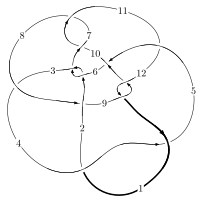
\includegraphics[width=112pt]{../../../GIT/diagram.site/Diagrams/png/1707_12a_0906.png}\\
\ \ \ A knot diagram\footnotemark}&
\allowdisplaybreaks
\textbf{Linearized knot diagam} \\
\cline{2-2}
 &
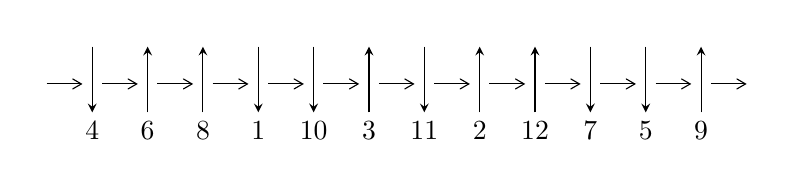
\begin{tikzpicture}[x=20pt, y=17pt]
	% nodes
	\node (C0) at (0, 0) {};
	\node (C1) at (1, 0) {};
	\node (C1U) at (1, +1) {};
	\node (C1D) at (1, -1) {4};

	\node (C2) at (2, 0) {};
	\node (C2U) at (2, +1) {};
	\node (C2D) at (2, -1) {6};

	\node (C3) at (3, 0) {};
	\node (C3U) at (3, +1) {};
	\node (C3D) at (3, -1) {8};

	\node (C4) at (4, 0) {};
	\node (C4U) at (4, +1) {};
	\node (C4D) at (4, -1) {1};

	\node (C5) at (5, 0) {};
	\node (C5U) at (5, +1) {};
	\node (C5D) at (5, -1) {10};

	\node (C6) at (6, 0) {};
	\node (C6U) at (6, +1) {};
	\node (C6D) at (6, -1) {3};

	\node (C7) at (7, 0) {};
	\node (C7U) at (7, +1) {};
	\node (C7D) at (7, -1) {11};

	\node (C8) at (8, 0) {};
	\node (C8U) at (8, +1) {};
	\node (C8D) at (8, -1) {2};

	\node (C9) at (9, 0) {};
	\node (C9U) at (9, +1) {};
	\node (C9D) at (9, -1) {12};

	\node (C10) at (10, 0) {};
	\node (C10U) at (10, +1) {};
	\node (C10D) at (10, -1) {7};

	\node (C11) at (11, 0) {};
	\node (C11U) at (11, +1) {};
	\node (C11D) at (11, -1) {5};

	\node (C12) at (12, 0) {};
	\node (C12U) at (12, +1) {};
	\node (C12D) at (12, -1) {9};
	\node (C13) at (13, 0) {};

	% arrows
	\draw[->,>={angle 60}]
	(C0) edge (C1) (C1) edge (C2) (C2) edge (C3) (C3) edge (C4) (C4) edge (C5) (C5) edge (C6) (C6) edge (C7) (C7) edge (C8) (C8) edge (C9) (C9) edge (C10) (C10) edge (C11) (C11) edge (C12) (C12) edge (C13) ;	\draw[->,>=stealth]
	(C1U) edge (C1D) (C2D) edge (C2U) (C3D) edge (C3U) (C4U) edge (C4D) (C5U) edge (C5D) (C6D) edge (C6U) (C7U) edge (C7D) (C8D) edge (C8U) (C9D) edge (C9U) (C10U) edge (C10D) (C11U) edge (C11D) (C12D) edge (C12U) ;
	\end{tikzpicture} \\
\hhline{~~} \\& 
\textbf{Solving Sequence} \\ \cline{2-2} 
 &
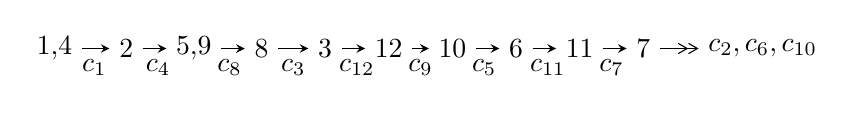
\begin{tikzpicture}[x=23pt, y=7pt]
	% node
	\node (A0) at (-1/8, 0) {1,4};
	\node (A1) at (1, 0) {2};
	\node (A2) at (33/16, 0) {5,9};
	\node (A3) at (25/8, 0) {8};
	\node (A4) at (33/8, 0) {3};
	\node (A5) at (41/8, 0) {12};
	\node (A6) at (49/8, 0) {10};
	\node (A7) at (57/8, 0) {6};
	\node (A8) at (65/8, 0) {11};
	\node (A9) at (73/8, 0) {7};
	\node (C1) at (1/2, -1) {$c_{1}$};
	\node (C2) at (3/2, -1) {$c_{4}$};
	\node (C3) at (21/8, -1) {$c_{8}$};
	\node (C4) at (29/8, -1) {$c_{3}$};
	\node (C5) at (37/8, -1) {$c_{12}$};
	\node (C6) at (45/8, -1) {$c_{9}$};
	\node (C7) at (53/8, -1) {$c_{5}$};
	\node (C8) at (61/8, -1) {$c_{11}$};
	\node (C9) at (69/8, -1) {$c_{7}$};
	\node (A10) at (11, 0) {$c_{2},c_{6},c_{10}$};

	% edge
	\draw[->,>=stealth]	
	(A0) edge (A1) (A1) edge (A2) (A2) edge (A3) (A3) edge (A4) (A4) edge (A5) (A5) edge (A6) (A6) edge (A7) (A7) edge (A8) (A8) edge (A9) ;
	\draw[->>,>={angle 60}]	
	(A9) edge (A10);
\end{tikzpicture} \\ 

\end{tabular} \\

\footnotetext{
The image of knot diagram is generated by the software ``\textbf{Draw programme}" developed by Andrew Bartholomew(\url{http://www.layer8.co.uk/maths/draw/index.htm\#Running-draw}), where we modified some parts for our purpose(\url{https://github.com/CATsTAILs/LinksPainter}).
}\phantom \\ \newline 
\centering \textbf{Ideals for irreducible components\footnotemark of $X_{\text{par}}$} 
 
\begin{align*}
I^u_{1}&=\langle 
3.04772\times10^{856} u^{165}+2.15325\times10^{857} u^{164}+\cdots+7.14027\times10^{856} b-2.56483\times10^{859},\\
\phantom{I^u_{1}}&\phantom{= \langle  }-5.81109\times10^{862} u^{165}-3.21459\times10^{863} u^{164}+\cdots+1.88142\times10^{863} a+1.42202\times10^{866},\\
\phantom{I^u_{1}}&\phantom{= \langle  }u^{166}+8 u^{165}+\cdots+2632 u+872\rangle \\
I^u_{2}&=\langle 
-2.55124\times10^{30} u^{37}+8.73175\times10^{29} u^{36}+\cdots+2.16094\times10^{30} b-2.67181\times10^{30},\\
\phantom{I^u_{2}}&\phantom{= \langle  }8.56010\times10^{31} u^{37}+4.54227\times10^{31} u^{36}+\cdots+3.94371\times10^{31} a+2.76795\times10^{32},\;u^{38}- u^{37}+\cdots-8 u+1\rangle \\
I^u_{3}&=\langle 
b^2+b u+u^2- b- u+2,\;- u^2+a-1,\;u^3- u^2+2 u-1\rangle \\
\\
\end{align*}
\raggedright * 3 irreducible components of $\dim_{\mathbb{C}}=0$, with total 210 representations.\\
\footnotetext{All coefficients of polynomials are rational numbers. But the coefficients are sometimes approximated in decimal forms when there is not enough margin.}
\newpage
\renewcommand{\arraystretch}{1}
\centering \section*{I. $I^u_{1}= \langle 3.05\times10^{856} u^{165}+2.15\times10^{857} u^{164}+\cdots+7.14\times10^{856} b-2.56\times10^{859},\;-5.81\times10^{862} u^{165}-3.21\times10^{863} u^{164}+\cdots+1.88\times10^{863} a+1.42\times10^{866},\;u^{166}+8 u^{165}+\cdots+2632 u+872 \rangle$}
\flushleft \textbf{(i) Arc colorings}\\
\begin{tabular}{m{7pt} m{180pt} m{7pt} m{180pt} }
\flushright $a_{1}=$&$\begin{pmatrix}1\\0\end{pmatrix}$ \\
\flushright $a_{4}=$&$\begin{pmatrix}0\\u\end{pmatrix}$ \\
\flushright $a_{2}=$&$\begin{pmatrix}1\\u^2\end{pmatrix}$ \\
\flushright $a_{5}=$&$\begin{pmatrix}- u\\u\end{pmatrix}$ \\
\flushright $a_{9}=$&$\begin{pmatrix}0.308868 u^{165}+1.70860 u^{164}+\cdots-1647.45 u-755.823\\-0.426835 u^{165}-3.01565 u^{164}+\cdots+488.904 u+359.207\end{pmatrix}$ \\
\flushright $a_{8}=$&$\begin{pmatrix}0.709267 u^{165}+5.10475 u^{164}+\cdots-399.199 u-450.266\\-0.801687 u^{165}-6.07418 u^{164}+\cdots-368.114 u+190.946\end{pmatrix}$ \\
\flushright $a_{3}=$&$\begin{pmatrix}1.66949 u^{165}+12.4962 u^{164}+\cdots+514.887 u-490.226\\-1.29994 u^{165}-9.74217 u^{164}+\cdots-506.050 u+346.274\end{pmatrix}$ \\
\flushright $a_{12}=$&$\begin{pmatrix}1.00412 u^{165}+8.54831 u^{164}+\cdots+3623.57 u+937.744\\-0.586007 u^{165}-5.28118 u^{164}+\cdots-2908.83 u-836.491\end{pmatrix}$ \\
\flushright $a_{10}=$&$\begin{pmatrix}-1.54406 u^{165}-10.8649 u^{164}+\cdots+1675.08 u+1229.26\\1.57472 u^{165}+11.1056 u^{164}+\cdots-1400.65 u-1149.74\end{pmatrix}$ \\
\flushright $a_{6}=$&$\begin{pmatrix}1.25092 u^{165}+9.70100 u^{164}+\cdots+1430.93 u+76.9177\\-1.55368 u^{165}-12.0162 u^{164}+\cdots-1799.48 u-58.1751\end{pmatrix}$ \\
\flushright $a_{11}=$&$\begin{pmatrix}0.700034 u^{165}+6.28921 u^{164}+\cdots+3463.72 u+1005.58\\-0.281919 u^{165}-3.02209 u^{164}+\cdots-2748.98 u-904.325\end{pmatrix}$ \\
\flushright $a_{7}=$&$\begin{pmatrix}0.277983 u^{165}+3.57812 u^{164}+\cdots+4227.48 u+1464.30\\-1.07064 u^{165}-9.95430 u^{164}+\cdots-5989.86 u-1805.10\end{pmatrix}$\\&\end{tabular}
\flushleft \textbf{(ii) Obstruction class $= -1$}\\~\\
\flushleft \textbf{(iii) Cusp Shapes $= -5.81941 u^{165}-45.7526 u^{164}+\cdots-8806.53 u-906.143$}\\~\\
\newpage\renewcommand{\arraystretch}{1}
\flushleft \textbf{(iv) u-Polynomials at the component}\newline \\
\begin{tabular}{m{50pt}|m{274pt}}
Crossings & \hspace{64pt}u-Polynomials at each crossing \\
\hline $$\begin{aligned}c_{1},c_{4}\end{aligned}$$&$\begin{aligned}
&u^{166}-8 u^{165}+\cdots-2632 u+872
\end{aligned}$\\
\hline $$\begin{aligned}c_{2},c_{6}\end{aligned}$$&$\begin{aligned}
&u^{166}-6 u^{165}+\cdots-44364 u+15032
\end{aligned}$\\
\hline $$\begin{aligned}c_{3}\end{aligned}$$&$\begin{aligned}
&u^{166}+u^{165}+\cdots+77004800 u+37093376
\end{aligned}$\\
\hline $$\begin{aligned}c_{5}\end{aligned}$$&$\begin{aligned}
&u^{166}- u^{165}+\cdots-77004800 u+37093376
\end{aligned}$\\
\hline $$\begin{aligned}c_{7},c_{10}\end{aligned}$$&$\begin{aligned}
&u^{166}+6 u^{165}+\cdots+44364 u+15032
\end{aligned}$\\
\hline $$\begin{aligned}c_{8}\end{aligned}$$&$\begin{aligned}
&u^{166}-2 u^{165}+\cdots+23296 u+6376
\end{aligned}$\\
\hline $$\begin{aligned}c_{9},c_{12}\end{aligned}$$&$\begin{aligned}
&u^{166}+8 u^{165}+\cdots+2632 u+872
\end{aligned}$\\
\hline $$\begin{aligned}c_{11}\end{aligned}$$&$\begin{aligned}
&u^{166}+2 u^{165}+\cdots-23296 u+6376
\end{aligned}$\\
\hline
\end{tabular}\\~\\
\newpage\renewcommand{\arraystretch}{1}
\flushleft \textbf{(v) Riley Polynomials at the component}\newline \\
\begin{tabular}{m{50pt}|m{274pt}}
Crossings & \hspace{64pt}Riley Polynomials at each crossing \\
\hline $$\begin{aligned}c_{1},c_{4},c_{9}\\c_{12}\end{aligned}$$&$\begin{aligned}
&y^{166}+112 y^{165}+\cdots+54967136 y+760384
\end{aligned}$\\
\hline $$\begin{aligned}c_{2},c_{6},c_{7}\\c_{10}\end{aligned}$$&$\begin{aligned}
&y^{166}-88 y^{165}+\cdots-10772707536 y+225961024
\end{aligned}$\\
\hline $$\begin{aligned}c_{3},c_{5}\end{aligned}$$&$\begin{aligned}
&y^{166}-37 y^{165}+\cdots-110732919839916032 y+1375918543077376
\end{aligned}$\\
\hline $$\begin{aligned}c_{8},c_{11}\end{aligned}$$&$\begin{aligned}
&y^{166}-4 y^{165}+\cdots+2251132064 y+40653376
\end{aligned}$\\
\hline
\end{tabular}\\~\\
\newpage\flushleft \textbf{(vi) Complex Volumes and Cusp Shapes}
$$\begin{array}{c|c|c}  
\text{Solutions to }I^u_{1}& \I (\text{vol} + \sqrt{-1}CS) & \text{Cusp shape}\\
 \hline 
\begin{aligned}
u &= \phantom{-}0.972169 + 0.218898 I \\
a &= -0.128892 + 0.159914 I \\
b &= \phantom{-}0.234140 + 1.328490 I\end{aligned}
 & -7.28993 - 0.80501 I & \phantom{-0.000000 } 0 \\ \hline\begin{aligned}
u &= \phantom{-}0.972169 - 0.218898 I \\
a &= -0.128892 - 0.159914 I \\
b &= \phantom{-}0.234140 - 1.328490 I\end{aligned}
 & -7.28993 + 0.80501 I & \phantom{-0.000000 } 0 \\ \hline\begin{aligned}
u &= -0.241874 + 0.958464 I \\
a &= -1.81538 + 0.81812 I \\
b &= \phantom{-}1.106070 - 0.249313 I\end{aligned}
 & -1.26280 + 2.02558 I & \phantom{-0.000000 } 0 \\ \hline\begin{aligned}
u &= -0.241874 - 0.958464 I \\
a &= -1.81538 - 0.81812 I \\
b &= \phantom{-}1.106070 + 0.249313 I\end{aligned}
 & -1.26280 - 2.02558 I & \phantom{-0.000000 } 0 \\ \hline\begin{aligned}
u &= -0.330909 + 0.958382 I \\
a &= \phantom{-}1.234160 + 0.600276 I \\
b &= -0.56010 - 1.49269 I\end{aligned}
 & \phantom{-}0.64081 + 2.61414 I & \phantom{-0.000000 } 0 \\ \hline\begin{aligned}
u &= -0.330909 - 0.958382 I \\
a &= \phantom{-}1.234160 - 0.600276 I \\
b &= -0.56010 + 1.49269 I\end{aligned}
 & \phantom{-}0.64081 - 2.61414 I & \phantom{-0.000000 } 0 \\ \hline\begin{aligned}
u &= \phantom{-}0.613798 + 0.813224 I \\
a &= -0.69358 - 1.37041 I \\
b &= \phantom{-}0.116888 - 1.252910 I\end{aligned}
 & -5.25563 - 2.26754 I & \phantom{-0.000000 } 0 \\ \hline\begin{aligned}
u &= \phantom{-}0.613798 - 0.813224 I \\
a &= -0.69358 + 1.37041 I \\
b &= \phantom{-}0.116888 + 1.252910 I\end{aligned}
 & -5.25563 + 2.26754 I & \phantom{-0.000000 } 0 \\ \hline\begin{aligned}
u &= -0.030127 + 1.025620 I \\
a &= -1.74054 - 0.44163 I \\
b &= \phantom{-}0.161139 - 0.843990 I\end{aligned}
 & \phantom{-}4.56133 + 2.80842 I & \phantom{-0.000000 } 0 \\ \hline\begin{aligned}
u &= -0.030127 - 1.025620 I \\
a &= -1.74054 + 0.44163 I \\
b &= \phantom{-}0.161139 + 0.843990 I\end{aligned}
 & \phantom{-}4.56133 - 2.80842 I & \phantom{-0.000000 } 0\\
 \hline 
 \end{array}$$\newpage$$\begin{array}{c|c|c}  
\text{Solutions to }I^u_{1}& \I (\text{vol} + \sqrt{-1}CS) & \text{Cusp shape}\\
 \hline 
\begin{aligned}
u &= -0.885024 + 0.524345 I \\
a &= \phantom{-}0.143825 + 0.269554 I \\
b &= -0.451443 + 0.448364 I\end{aligned}
 & \phantom{-}1.42629 - 4.21693 I & \phantom{-0.000000 } 0 \\ \hline\begin{aligned}
u &= -0.885024 - 0.524345 I \\
a &= \phantom{-}0.143825 - 0.269554 I \\
b &= -0.451443 - 0.448364 I\end{aligned}
 & \phantom{-}1.42629 + 4.21693 I & \phantom{-0.000000 } 0 \\ \hline\begin{aligned}
u &= -0.127639 + 0.955130 I \\
a &= -0.939256 + 0.779728 I \\
b &= \phantom{-}0.16705 + 1.40981 I\end{aligned}
 & -4.33829 + 4.25319 I & \phantom{-0.000000 } 0 \\ \hline\begin{aligned}
u &= -0.127639 - 0.955130 I \\
a &= -0.939256 - 0.779728 I \\
b &= \phantom{-}0.16705 - 1.40981 I\end{aligned}
 & -4.33829 - 4.25319 I & \phantom{-0.000000 } 0 \\ \hline\begin{aligned}
u &= -0.225299 + 0.936493 I \\
a &= \phantom{-}1.352360 + 0.100036 I \\
b &= -0.486351 - 1.236260 I\end{aligned}
 & \phantom{-}0.64887 + 2.89892 I & \phantom{-0.000000 } 0 \\ \hline\begin{aligned}
u &= -0.225299 - 0.936493 I \\
a &= \phantom{-}1.352360 - 0.100036 I \\
b &= -0.486351 + 1.236260 I\end{aligned}
 & \phantom{-}0.64887 - 2.89892 I & \phantom{-0.000000 } 0 \\ \hline\begin{aligned}
u &= \phantom{-}0.209745 + 1.023240 I \\
a &= \phantom{-}1.02484 - 1.59523 I \\
b &= -0.249301 + 1.027720 I\end{aligned}
 & -1.94689 - 3.53576 I & \phantom{-0.000000 } 0 \\ \hline\begin{aligned}
u &= \phantom{-}0.209745 - 1.023240 I \\
a &= \phantom{-}1.02484 + 1.59523 I \\
b &= -0.249301 - 1.027720 I\end{aligned}
 & -1.94689 + 3.53576 I & \phantom{-0.000000 } 0 \\ \hline\begin{aligned}
u &= \phantom{-}0.152380 + 0.931757 I \\
a &= -0.88458 - 1.19968 I \\
b &= \phantom{-}0.78153 + 1.70359 I\end{aligned}
 & -2.50839 - 0.97139 I & \phantom{-0.000000 } 0 \\ \hline\begin{aligned}
u &= \phantom{-}0.152380 - 0.931757 I \\
a &= -0.88458 + 1.19968 I \\
b &= \phantom{-}0.78153 - 1.70359 I\end{aligned}
 & -2.50839 + 0.97139 I & \phantom{-0.000000 } 0\\
 \hline 
 \end{array}$$\newpage$$\begin{array}{c|c|c}  
\text{Solutions to }I^u_{1}& \I (\text{vol} + \sqrt{-1}CS) & \text{Cusp shape}\\
 \hline 
\begin{aligned}
u &= \phantom{-}0.249301 + 1.027720 I \\
a &= \phantom{-}0.454155 + 0.833480 I \\
b &= -0.209745 + 1.023240 I\end{aligned}
 & \phantom{-}1.94689 - 3.53576 I & \phantom{-0.000000 } 0 \\ \hline\begin{aligned}
u &= \phantom{-}0.249301 - 1.027720 I \\
a &= \phantom{-}0.454155 - 0.833480 I \\
b &= -0.209745 - 1.023240 I\end{aligned}
 & \phantom{-}1.94689 + 3.53576 I & \phantom{-0.000000 } 0 \\ \hline\begin{aligned}
u &= \phantom{-}0.035069 + 1.059860 I \\
a &= \phantom{-}2.26454 - 0.47380 I \\
b &= -0.582937 + 0.928006 I\end{aligned}
 & \phantom{-}4.95016 - 2.52119 I & \phantom{-0.000000 } 0 \\ \hline\begin{aligned}
u &= \phantom{-}0.035069 - 1.059860 I \\
a &= \phantom{-}2.26454 + 0.47380 I \\
b &= -0.582937 - 0.928006 I\end{aligned}
 & \phantom{-}4.95016 + 2.52119 I & \phantom{-0.000000 } 0 \\ \hline\begin{aligned}
u &= -0.651241 + 0.667306 I \\
a &= \phantom{-}0.575706 + 0.364985 I \\
b &= \phantom{-}0.339015 - 1.328620 I\end{aligned}
 & -6.62966 - 2.49532 I & \phantom{-0.000000 } 0 \\ \hline\begin{aligned}
u &= -0.651241 - 0.667306 I \\
a &= \phantom{-}0.575706 - 0.364985 I \\
b &= \phantom{-}0.339015 + 1.328620 I\end{aligned}
 & -6.62966 + 2.49532 I & \phantom{-0.000000 } 0 \\ \hline\begin{aligned}
u &= -0.447824 + 0.970612 I \\
a &= -1.72043 - 0.13388 I \\
b &= \phantom{-}0.63804 + 1.35560 I\end{aligned}
 & -5.64838 + 6.76788 I & \phantom{-0.000000 } 0 \\ \hline\begin{aligned}
u &= -0.447824 - 0.970612 I \\
a &= -1.72043 + 0.13388 I \\
b &= \phantom{-}0.63804 - 1.35560 I\end{aligned}
 & -5.64838 - 6.76788 I & \phantom{-0.000000 } 0 \\ \hline\begin{aligned}
u &= \phantom{-}1.047770 + 0.258314 I \\
a &= -0.212607 + 0.061679 I \\
b &= -0.330148 - 1.199420 I\end{aligned}
 & -3.34359 + 1.96570 I & \phantom{-0.000000 } 0 \\ \hline\begin{aligned}
u &= \phantom{-}1.047770 - 0.258314 I \\
a &= -0.212607 - 0.061679 I \\
b &= -0.330148 + 1.199420 I\end{aligned}
 & -3.34359 - 1.96570 I & \phantom{-0.000000 } 0\\
 \hline 
 \end{array}$$\newpage$$\begin{array}{c|c|c}  
\text{Solutions to }I^u_{1}& \I (\text{vol} + \sqrt{-1}CS) & \text{Cusp shape}\\
 \hline 
\begin{aligned}
u &= \phantom{-}0.860323 + 0.669737 I \\
a &= \phantom{-}0.037789 - 0.360133 I \\
b &= \phantom{-}0.461677 + 1.274220 I\end{aligned}
 & -4.59764 + 5.27559 I & \phantom{-0.000000 } 0 \\ \hline\begin{aligned}
u &= \phantom{-}0.860323 - 0.669737 I \\
a &= \phantom{-}0.037789 + 0.360133 I \\
b &= \phantom{-}0.461677 - 1.274220 I\end{aligned}
 & -4.59764 - 5.27559 I & \phantom{-0.000000 } 0 \\ \hline\begin{aligned}
u &= \phantom{-}0.061638 + 0.907243 I \\
a &= \phantom{-}0.780592 - 0.464704 I \\
b &= -0.23918 - 1.46071 I\end{aligned}
 & -2.66064 + 2.48196 I & \phantom{-0.000000 } 0 \\ \hline\begin{aligned}
u &= \phantom{-}0.061638 - 0.907243 I \\
a &= \phantom{-}0.780592 + 0.464704 I \\
b &= -0.23918 + 1.46071 I\end{aligned}
 & -2.66064 - 2.48196 I & \phantom{-0.000000 } 0 \\ \hline\begin{aligned}
u &= \phantom{-}0.582937 + 0.928006 I \\
a &= \phantom{-}1.59448 + 0.54639 I \\
b &= -0.035069 + 1.059860 I\end{aligned}
 & -4.95016 - 2.52119 I & \phantom{-0.000000 } 0 \\ \hline\begin{aligned}
u &= \phantom{-}0.582937 - 0.928006 I \\
a &= \phantom{-}1.59448 - 0.54639 I \\
b &= -0.035069 - 1.059860 I\end{aligned}
 & -4.95016 + 2.52119 I & \phantom{-0.000000 } 0 \\ \hline\begin{aligned}
u &= \phantom{-}0.130373 + 1.088470 I \\
a &= -2.40675 - 0.57766 I \\
b &= \phantom{-}0.363797 - 1.133890 I\end{aligned}
 & \phantom{-}1.31493 - 9.17596 I & \phantom{-0.000000 } 0 \\ \hline\begin{aligned}
u &= \phantom{-}0.130373 - 1.088470 I \\
a &= -2.40675 + 0.57766 I \\
b &= \phantom{-}0.363797 + 1.133890 I\end{aligned}
 & \phantom{-}1.31493 + 9.17596 I & \phantom{-0.000000 } 0 \\ \hline\begin{aligned}
u &= -0.142227 + 0.890446 I \\
a &= -0.24139 + 1.58897 I \\
b &= \phantom{-}0.32729 - 2.09186 I\end{aligned}
 & -2.01341 + 6.35063 I & \phantom{-0.000000 } 0 \\ \hline\begin{aligned}
u &= -0.142227 - 0.890446 I \\
a &= -0.24139 - 1.58897 I \\
b &= \phantom{-}0.32729 + 2.09186 I\end{aligned}
 & -2.01341 - 6.35063 I & \phantom{-0.000000 } 0\\
 \hline 
 \end{array}$$\newpage$$\begin{array}{c|c|c}  
\text{Solutions to }I^u_{1}& \I (\text{vol} + \sqrt{-1}CS) & \text{Cusp shape}\\
 \hline 
\begin{aligned}
u &= -1.101570 + 0.069081 I \\
a &= \phantom{-}0.228295 - 0.259670 I \\
b &= -0.385385 - 1.286770 I\end{aligned}
 & -1.48964 + 7.78003 I & \phantom{-0.000000 } 0 \\ \hline\begin{aligned}
u &= -1.101570 - 0.069081 I \\
a &= \phantom{-}0.228295 + 0.259670 I \\
b &= -0.385385 + 1.286770 I\end{aligned}
 & -1.48964 - 7.78003 I & \phantom{-0.000000 } 0 \\ \hline\begin{aligned}
u &= \phantom{-}1.109350 + 0.049474 I \\
a &= \phantom{-}0.002103 + 0.278265 I \\
b &= -0.240939 + 1.226760 I\end{aligned}
 & -4.28618 - 2.77563 I & \phantom{-0.000000 } 0 \\ \hline\begin{aligned}
u &= \phantom{-}1.109350 - 0.049474 I \\
a &= \phantom{-}0.002103 - 0.278265 I \\
b &= -0.240939 - 1.226760 I\end{aligned}
 & -4.28618 + 2.77563 I & \phantom{-0.000000 } 0 \\ \hline\begin{aligned}
u &= \phantom{-}0.401620 + 0.778058 I \\
a &= -1.78845 - 0.73107 I \\
b &= \phantom{-}0.832421 + 0.085376 I\end{aligned}
 & -0.645618 + 0.585336 I & \phantom{-0.000000 } 0 \\ \hline\begin{aligned}
u &= \phantom{-}0.401620 - 0.778058 I \\
a &= -1.78845 + 0.73107 I \\
b &= \phantom{-}0.832421 - 0.085376 I\end{aligned}
 & -0.645618 - 0.585336 I & \phantom{-0.000000 } 0 \\ \hline\begin{aligned}
u &= -1.106070 + 0.249313 I \\
a &= -0.162926 - 0.775764 I \\
b &= \phantom{-}0.241874 - 0.958464 I\end{aligned}
 & \phantom{-}1.26280 - 2.02558 I & \phantom{-0.000000 } 0 \\ \hline\begin{aligned}
u &= -1.106070 - 0.249313 I \\
a &= -0.162926 + 0.775764 I \\
b &= \phantom{-}0.241874 + 0.958464 I\end{aligned}
 & \phantom{-}1.26280 + 2.02558 I & \phantom{-0.000000 } 0 \\ \hline\begin{aligned}
u &= \phantom{-}0.083335 + 0.860633 I \\
a &= -2.07119 + 1.07012 I \\
b &= \phantom{-}1.32235 - 0.96830 I\end{aligned}
 & -2.88532 - 0.42811 I & \phantom{-0.000000 } 0 \\ \hline\begin{aligned}
u &= \phantom{-}0.083335 - 0.860633 I \\
a &= -2.07119 - 1.07012 I \\
b &= \phantom{-}1.32235 + 0.96830 I\end{aligned}
 & -2.88532 + 0.42811 I & \phantom{-0.000000 } 0\\
 \hline 
 \end{array}$$\newpage$$\begin{array}{c|c|c}  
\text{Solutions to }I^u_{1}& \I (\text{vol} + \sqrt{-1}CS) & \text{Cusp shape}\\
 \hline 
\begin{aligned}
u &= -0.161139 + 0.843990 I \\
a &= \phantom{-}2.10569 + 1.21665 I \\
b &= \phantom{-}0.030127 - 1.025620 I\end{aligned}
 & -4.56133 - 2.80842 I & \phantom{-0.000000 } 0 \\ \hline\begin{aligned}
u &= -0.161139 - 0.843990 I \\
a &= \phantom{-}2.10569 - 1.21665 I \\
b &= \phantom{-}0.030127 + 1.025620 I\end{aligned}
 & -4.56133 + 2.80842 I & \phantom{-0.000000 } 0 \\ \hline\begin{aligned}
u &= \phantom{-}0.614309 + 0.973766 I \\
a &= -1.68275 + 0.10562 I \\
b &= \phantom{-}0.73446 - 1.26312 I\end{aligned}
 & -3.55161 - 10.76260 I & \phantom{-0.000000 } 0 \\ \hline\begin{aligned}
u &= \phantom{-}0.614309 - 0.973766 I \\
a &= -1.68275 - 0.10562 I \\
b &= \phantom{-}0.73446 + 1.26312 I\end{aligned}
 & -3.55161 + 10.76260 I & \phantom{-0.000000 } 0 \\ \hline\begin{aligned}
u &= \phantom{-}0.696817 + 0.928767 I \\
a &= -0.069883 - 0.256345 I \\
b &= -0.116062 - 0.135620 I\end{aligned}
 & -1.19072 - 1.66992 I & \phantom{-0.000000 } 0 \\ \hline\begin{aligned}
u &= \phantom{-}0.696817 - 0.928767 I \\
a &= -0.069883 + 0.256345 I \\
b &= -0.116062 + 0.135620 I\end{aligned}
 & -1.19072 + 1.66992 I & \phantom{-0.000000 } 0 \\ \hline\begin{aligned}
u &= -0.832421 + 0.085376 I \\
a &= \phantom{-}0.018474 + 1.207020 I \\
b &= -0.401620 + 0.778058 I\end{aligned}
 & \phantom{-}0.645618 + 0.585336 I & \phantom{-0.000000 } 0 \\ \hline\begin{aligned}
u &= -0.832421 - 0.085376 I \\
a &= \phantom{-}0.018474 - 1.207020 I \\
b &= -0.401620 - 0.778058 I\end{aligned}
 & \phantom{-}0.645618 - 0.585336 I & \phantom{-0.000000 } 0 \\ \hline\begin{aligned}
u &= \phantom{-}0.788236 + 0.244072 I \\
a &= \phantom{-}0.012371 + 0.586664 I \\
b &= \phantom{-}0.494958 - 0.132987 I\end{aligned}
 & -3.03351 - 3.67994 I & \phantom{-0.000000 } 0 \\ \hline\begin{aligned}
u &= \phantom{-}0.788236 - 0.244072 I \\
a &= \phantom{-}0.012371 - 0.586664 I \\
b &= \phantom{-}0.494958 + 0.132987 I\end{aligned}
 & -3.03351 + 3.67994 I & \phantom{-0.000000 } 0\\
 \hline 
 \end{array}$$\newpage$$\begin{array}{c|c|c}  
\text{Solutions to }I^u_{1}& \I (\text{vol} + \sqrt{-1}CS) & \text{Cusp shape}\\
 \hline 
\begin{aligned}
u &= -0.034081 + 0.821473 I \\
a &= \phantom{-}3.09960 - 0.54004 I \\
b &= \phantom{-}0.034081 + 0.821473 I\end{aligned}
 & \phantom{-0.000000 -}8.51377 I & \phantom{-0.000000 } 0 \\ \hline\begin{aligned}
u &= -0.034081 - 0.821473 I \\
a &= \phantom{-}3.09960 + 0.54004 I \\
b &= \phantom{-}0.034081 - 0.821473 I\end{aligned}
 & \phantom{-0.000000 } -8.51377 I & \phantom{-0.000000 } 0 \\ \hline\begin{aligned}
u &= \phantom{-}0.303969 + 1.143130 I \\
a &= \phantom{-}1.37878 - 0.74323 I \\
b &= -0.78329 + 1.51303 I\end{aligned}
 & \phantom{-}0.84891 - 6.85717 I & \phantom{-0.000000 } 0 \\ \hline\begin{aligned}
u &= \phantom{-}0.303969 - 1.143130 I \\
a &= \phantom{-}1.37878 + 0.74323 I \\
b &= -0.78329 - 1.51303 I\end{aligned}
 & \phantom{-}0.84891 + 6.85717 I & \phantom{-0.000000 } 0 \\ \hline\begin{aligned}
u &= -0.363797 + 1.133890 I \\
a &= \phantom{-}2.36613 + 0.64895 I \\
b &= -0.130373 - 1.088470 I\end{aligned}
 & -1.31493 + 9.17596 I & \phantom{-0.000000 } 0 \\ \hline\begin{aligned}
u &= -0.363797 - 1.133890 I \\
a &= \phantom{-}2.36613 - 0.64895 I \\
b &= -0.130373 + 1.088470 I\end{aligned}
 & -1.31493 - 9.17596 I & \phantom{-0.000000 } 0 \\ \hline\begin{aligned}
u &= \phantom{-}0.198308 + 1.176710 I \\
a &= \phantom{-}1.71393 - 0.52899 I \\
b &= -1.123230 + 0.576311 I\end{aligned}
 & \phantom{-}4.15083 - 3.32222 I & \phantom{-0.000000 } 0 \\ \hline\begin{aligned}
u &= \phantom{-}0.198308 - 1.176710 I \\
a &= \phantom{-}1.71393 + 0.52899 I \\
b &= -1.123230 - 0.576311 I\end{aligned}
 & \phantom{-}4.15083 + 3.32222 I & \phantom{-0.000000 } 0 \\ \hline\begin{aligned}
u &= -0.233186 + 0.768133 I \\
a &= -1.86686 - 1.12090 I \\
b &= \phantom{-}0.87930 + 1.27832 I\end{aligned}
 & -2.05570 - 4.32127 I & \phantom{-0.000000 } 0 \\ \hline\begin{aligned}
u &= -0.233186 - 0.768133 I \\
a &= -1.86686 + 1.12090 I \\
b &= \phantom{-}0.87930 - 1.27832 I\end{aligned}
 & -2.05570 + 4.32127 I & \phantom{-0.000000 } 0\\
 \hline 
 \end{array}$$\newpage$$\begin{array}{c|c|c}  
\text{Solutions to }I^u_{1}& \I (\text{vol} + \sqrt{-1}CS) & \text{Cusp shape}\\
 \hline 
\begin{aligned}
u &= -0.160540 + 0.784851 I \\
a &= -1.48487 - 0.10512 I \\
b &= \phantom{-}0.160540 + 0.784851 I\end{aligned}
 & \phantom{-0.000000 } -0.664448 I & \phantom{-0.000000 } 0 \\ \hline\begin{aligned}
u &= -0.160540 - 0.784851 I \\
a &= -1.48487 + 0.10512 I \\
b &= \phantom{-}0.160540 - 0.784851 I\end{aligned}
 & \phantom{-0.000000 -}0.664448 I & \phantom{-0.000000 } 0 \\ \hline\begin{aligned}
u &= -0.743499 + 0.235712 I \\
a &= -0.662425 - 0.472261 I \\
b &= \phantom{-}0.304555 - 0.177362 I\end{aligned}
 & \phantom{-}3.05344 - 0.37163 I & \phantom{-0.000000 } 0 \\ \hline\begin{aligned}
u &= -0.743499 - 0.235712 I \\
a &= -0.662425 + 0.472261 I \\
b &= \phantom{-}0.304555 + 0.177362 I\end{aligned}
 & \phantom{-}3.05344 + 0.37163 I & \phantom{-0.000000 } 0 \\ \hline\begin{aligned}
u &= \phantom{-}0.330148 + 1.199420 I \\
a &= \phantom{-}1.091160 + 0.071251 I \\
b &= -1.047770 - 0.258314 I\end{aligned}
 & \phantom{-}3.34359 - 1.96570 I & \phantom{-0.000000 } 0 \\ \hline\begin{aligned}
u &= \phantom{-}0.330148 - 1.199420 I \\
a &= \phantom{-}1.091160 - 0.071251 I \\
b &= -1.047770 + 0.258314 I\end{aligned}
 & \phantom{-}3.34359 + 1.96570 I & \phantom{-0.000000 } 0 \\ \hline\begin{aligned}
u &= -0.719261 + 0.232376 I \\
a &= \phantom{-}0.020514 - 0.471466 I \\
b &= \phantom{-}0.385001 - 1.327700 I\end{aligned}
 & -7.76532 - 3.84221 I & \phantom{-0.000000 } 0 \\ \hline\begin{aligned}
u &= -0.719261 - 0.232376 I \\
a &= \phantom{-}0.020514 + 0.471466 I \\
b &= \phantom{-}0.385001 + 1.327700 I\end{aligned}
 & -7.76532 + 3.84221 I & \phantom{-0.000000 } 0 \\ \hline\begin{aligned}
u &= \phantom{-}0.240939 + 1.226760 I \\
a &= \phantom{-}1.353480 - 0.010847 I \\
b &= -1.109350 + 0.049474 I\end{aligned}
 & \phantom{-}4.28618 - 2.77563 I & \phantom{-0.000000 } 0 \\ \hline\begin{aligned}
u &= \phantom{-}0.240939 - 1.226760 I \\
a &= \phantom{-}1.353480 + 0.010847 I \\
b &= -1.109350 - 0.049474 I\end{aligned}
 & \phantom{-}4.28618 + 2.77563 I & \phantom{-0.000000 } 0\\
 \hline 
 \end{array}$$\newpage$$\begin{array}{c|c|c}  
\text{Solutions to }I^u_{1}& \I (\text{vol} + \sqrt{-1}CS) & \text{Cusp shape}\\
 \hline 
\begin{aligned}
u &= -0.116888 + 1.252910 I \\
a &= \phantom{-}1.77651 + 1.25446 I \\
b &= -0.613798 - 0.813224 I\end{aligned}
 & \phantom{-}5.25563 + 2.26754 I & \phantom{-0.000000 } 0 \\ \hline\begin{aligned}
u &= -0.116888 - 1.252910 I \\
a &= \phantom{-}1.77651 - 1.25446 I \\
b &= -0.613798 + 0.813224 I\end{aligned}
 & \phantom{-}5.25563 - 2.26754 I & \phantom{-0.000000 } 0 \\ \hline\begin{aligned}
u &= \phantom{-}1.123230 + 0.576311 I \\
a &= \phantom{-}0.211423 + 0.518704 I \\
b &= -0.198308 + 1.176710 I\end{aligned}
 & -4.15083 - 3.32222 I & \phantom{-0.000000 } 0 \\ \hline\begin{aligned}
u &= \phantom{-}1.123230 - 0.576311 I \\
a &= \phantom{-}0.211423 - 0.518704 I \\
b &= -0.198308 - 1.176710 I\end{aligned}
 & -4.15083 + 3.32222 I & \phantom{-0.000000 } 0 \\ \hline\begin{aligned}
u &= -0.310070 + 1.224610 I \\
a &= \phantom{-}1.61977 - 0.31229 I \\
b &= -1.348560 + 0.102625 I\end{aligned}
 & \phantom{-}6.97620 + 6.78564 I & \phantom{-0.000000 } 0 \\ \hline\begin{aligned}
u &= -0.310070 - 1.224610 I \\
a &= \phantom{-}1.61977 + 0.31229 I \\
b &= -1.348560 - 0.102625 I\end{aligned}
 & \phantom{-}6.97620 - 6.78564 I & \phantom{-0.000000 } 0 \\ \hline\begin{aligned}
u &= -0.686445 + 0.265915 I \\
a &= -1.052380 - 0.012259 I \\
b &= -0.069590 + 1.294380 I\end{aligned}
 & -1.29336 + 1.14631 I & \phantom{-0.000000 } 0 \\ \hline\begin{aligned}
u &= -0.686445 - 0.265915 I \\
a &= -1.052380 + 0.012259 I \\
b &= -0.069590 - 1.294380 I\end{aligned}
 & -1.29336 - 1.14631 I & \phantom{-0.000000 } 0 \\ \hline\begin{aligned}
u &= -0.406135 + 1.201730 I \\
a &= -1.87282 - 0.36960 I \\
b &= \phantom{-}0.58817 + 1.29969 I\end{aligned}
 & -4.73323 + 8.05445 I & \phantom{-0.000000 } 0 \\ \hline\begin{aligned}
u &= -0.406135 - 1.201730 I \\
a &= -1.87282 + 0.36960 I \\
b &= \phantom{-}0.58817 - 1.29969 I\end{aligned}
 & -4.73323 - 8.05445 I & \phantom{-0.000000 } 0\\
 \hline 
 \end{array}$$\newpage$$\begin{array}{c|c|c}  
\text{Solutions to }I^u_{1}& \I (\text{vol} + \sqrt{-1}CS) & \text{Cusp shape}\\
 \hline 
\begin{aligned}
u &= -0.714302 + 0.140698 I \\
a &= -0.166511 - 1.038200 I \\
b &= \phantom{-}0.714302 + 0.140698 I\end{aligned}
 & \phantom{-0.000000 -}9.66190 I & \phantom{-0.000000 } 0 \\ \hline\begin{aligned}
u &= -0.714302 - 0.140698 I \\
a &= -0.166511 + 1.038200 I \\
b &= \phantom{-}0.714302 - 0.140698 I\end{aligned}
 & \phantom{-0.000000 } -9.66190 I & \phantom{-0.000000 } 0 \\ \hline\begin{aligned}
u &= -1.280860 + 0.073525 I \\
a &= -0.177460 - 0.212483 I \\
b &= \phantom{-}0.409078 - 1.266050 I\end{aligned}
 & -4.1077 - 13.8043 I & \phantom{-0.000000 } 0 \\ \hline\begin{aligned}
u &= -1.280860 - 0.073525 I \\
a &= -0.177460 + 0.212483 I \\
b &= \phantom{-}0.409078 + 1.266050 I\end{aligned}
 & -4.1077 + 13.8043 I & \phantom{-0.000000 } 0 \\ \hline\begin{aligned}
u &= \phantom{-}0.069590 + 1.294380 I \\
a &= -0.925594 + 0.281853 I \\
b &= \phantom{-}0.686445 + 0.265915 I\end{aligned}
 & \phantom{-}1.29336 + 1.14631 I & \phantom{-0.000000 } 0 \\ \hline\begin{aligned}
u &= \phantom{-}0.069590 - 1.294380 I \\
a &= -0.925594 - 0.281853 I \\
b &= \phantom{-}0.686445 - 0.265915 I\end{aligned}
 & \phantom{-}1.29336 - 1.14631 I & \phantom{-0.000000 } 0 \\ \hline\begin{aligned}
u &= \phantom{-}0.067307 + 1.322720 I \\
a &= -0.774104 - 1.111060 I \\
b &= \phantom{-}0.482054 + 0.306015 I\end{aligned}
 & \phantom{-}3.80938 - 5.65587 I & \phantom{-0.000000 } 0 \\ \hline\begin{aligned}
u &= \phantom{-}0.067307 - 1.322720 I \\
a &= -0.774104 + 1.111060 I \\
b &= \phantom{-}0.482054 - 0.306015 I\end{aligned}
 & \phantom{-}3.80938 + 5.65587 I & \phantom{-0.000000 } 0 \\ \hline\begin{aligned}
u &= \phantom{-}0.486351 + 1.236260 I \\
a &= -0.986871 + 0.314652 I \\
b &= \phantom{-}0.225299 - 0.936493 I\end{aligned}
 & -0.64887 - 2.89892 I & \phantom{-0.000000 } 0 \\ \hline\begin{aligned}
u &= \phantom{-}0.486351 - 1.236260 I \\
a &= -0.986871 - 0.314652 I \\
b &= \phantom{-}0.225299 + 0.936493 I\end{aligned}
 & -0.64887 + 2.89892 I & \phantom{-0.000000 } 0\\
 \hline 
 \end{array}$$\newpage$$\begin{array}{c|c|c}  
\text{Solutions to }I^u_{1}& \I (\text{vol} + \sqrt{-1}CS) & \text{Cusp shape}\\
 \hline 
\begin{aligned}
u &= -0.409078 + 1.266050 I \\
a &= -1.41004 + 0.30714 I \\
b &= \phantom{-}1.280860 - 0.073525 I\end{aligned}
 & \phantom{-}4.1077 + 13.8043 I & \phantom{-0.000000 } 0 \\ \hline\begin{aligned}
u &= -0.409078 - 1.266050 I \\
a &= -1.41004 - 0.30714 I \\
b &= \phantom{-}1.280860 + 0.073525 I\end{aligned}
 & \phantom{-}4.1077 - 13.8043 I & \phantom{-0.000000 } 0 \\ \hline\begin{aligned}
u &= \phantom{-}0.534347 + 1.228490 I \\
a &= -1.57597 + 0.40557 I \\
b &= \phantom{-}0.525199 - 1.270700 I\end{aligned}
 & -4.11997 - 4.57380 I & \phantom{-0.000000 } 0 \\ \hline\begin{aligned}
u &= \phantom{-}0.534347 - 1.228490 I \\
a &= -1.57597 - 0.40557 I \\
b &= \phantom{-}0.525199 + 1.270700 I\end{aligned}
 & -4.11997 + 4.57380 I & \phantom{-0.000000 } 0 \\ \hline\begin{aligned}
u &= \phantom{-}0.385385 + 1.286770 I \\
a &= -1.266930 - 0.161940 I \\
b &= \phantom{-}1.101570 - 0.069081 I\end{aligned}
 & \phantom{-}1.48964 - 7.78003 I & \phantom{-0.000000 } 0 \\ \hline\begin{aligned}
u &= \phantom{-}0.385385 - 1.286770 I \\
a &= -1.266930 + 0.161940 I \\
b &= \phantom{-}1.101570 + 0.069081 I\end{aligned}
 & \phantom{-}1.48964 + 7.78003 I & \phantom{-0.000000 } 0 \\ \hline\begin{aligned}
u &= -0.234140 + 1.328490 I \\
a &= \phantom{-}1.044440 - 0.352307 I \\
b &= -0.972169 + 0.218898 I\end{aligned}
 & \phantom{-}7.28993 - 0.80501 I & \phantom{-0.000000 } 0 \\ \hline\begin{aligned}
u &= -0.234140 - 1.328490 I \\
a &= \phantom{-}1.044440 + 0.352307 I \\
b &= -0.972169 - 0.218898 I\end{aligned}
 & \phantom{-}7.28993 + 0.80501 I & \phantom{-0.000000 } 0 \\ \hline\begin{aligned}
u &= \phantom{-}1.348560 + 0.102625 I \\
a &= -0.105012 + 0.302490 I \\
b &= \phantom{-}0.310070 + 1.224610 I\end{aligned}
 & -6.97620 + 6.78564 I & \phantom{-0.000000 } 0 \\ \hline\begin{aligned}
u &= \phantom{-}1.348560 - 0.102625 I \\
a &= -0.105012 - 0.302490 I \\
b &= \phantom{-}0.310070 - 1.224610 I\end{aligned}
 & -6.97620 - 6.78564 I & \phantom{-0.000000 } 0\\
 \hline 
 \end{array}$$\newpage$$\begin{array}{c|c|c}  
\text{Solutions to }I^u_{1}& \I (\text{vol} + \sqrt{-1}CS) & \text{Cusp shape}\\
 \hline 
\begin{aligned}
u &= -0.461677 + 1.274220 I \\
a &= \phantom{-}0.731739 - 0.408347 I \\
b &= -0.860323 + 0.669737 I\end{aligned}
 & \phantom{-}4.59764 + 5.27559 I & \phantom{-0.000000 } 0 \\ \hline\begin{aligned}
u &= -0.461677 - 1.274220 I \\
a &= \phantom{-}0.731739 + 0.408347 I \\
b &= -0.860323 - 0.669737 I\end{aligned}
 & \phantom{-}4.59764 - 5.27559 I & \phantom{-0.000000 } 0 \\ \hline\begin{aligned}
u &= \phantom{-}0.451443 + 0.448364 I \\
a &= -0.766158 - 1.003790 I \\
b &= \phantom{-}0.885024 + 0.524345 I\end{aligned}
 & -1.42629 - 4.21693 I & \phantom{-0.000000 } 0 \\ \hline\begin{aligned}
u &= \phantom{-}0.451443 - 0.448364 I \\
a &= -0.766158 + 1.003790 I \\
b &= \phantom{-}0.885024 - 0.524345 I\end{aligned}
 & -1.42629 + 4.21693 I & \phantom{-0.000000 } 0 \\ \hline\begin{aligned}
u &= -0.339015 + 1.328620 I \\
a &= -0.866270 + 0.256667 I \\
b &= \phantom{-}0.651241 - 0.667306 I\end{aligned}
 & \phantom{-}6.62966 + 2.49532 I & \phantom{-0.000000 } 0 \\ \hline\begin{aligned}
u &= -0.339015 - 1.328620 I \\
a &= -0.866270 - 0.256667 I \\
b &= \phantom{-}0.651241 + 0.667306 I\end{aligned}
 & \phantom{-}6.62966 - 2.49532 I & \phantom{-0.000000 } 0 \\ \hline\begin{aligned}
u &= -0.525199 + 1.270700 I \\
a &= \phantom{-}1.317640 - 0.150072 I \\
b &= -0.534347 - 1.228490 I\end{aligned}
 & \phantom{-}4.11997 + 4.57380 I & \phantom{-0.000000 } 0 \\ \hline\begin{aligned}
u &= -0.525199 - 1.270700 I \\
a &= \phantom{-}1.317640 + 0.150072 I \\
b &= -0.534347 + 1.228490 I\end{aligned}
 & \phantom{-}4.11997 - 4.57380 I & \phantom{-0.000000 } 0 \\ \hline\begin{aligned}
u &= -0.385001 + 1.327700 I \\
a &= -0.939073 + 0.367520 I \\
b &= \phantom{-}0.719261 - 0.232376 I\end{aligned}
 & \phantom{-}7.76532 + 3.84221 I & \phantom{-0.000000 } 0 \\ \hline\begin{aligned}
u &= -0.385001 - 1.327700 I \\
a &= -0.939073 - 0.367520 I \\
b &= \phantom{-}0.719261 + 0.232376 I\end{aligned}
 & \phantom{-}7.76532 - 3.84221 I & \phantom{-0.000000 } 0\\
 \hline 
 \end{array}$$\newpage$$\begin{array}{c|c|c}  
\text{Solutions to }I^u_{1}& \I (\text{vol} + \sqrt{-1}CS) & \text{Cusp shape}\\
 \hline 
\begin{aligned}
u &= -0.16705 + 1.40981 I \\
a &= -0.87657 - 1.30961 I \\
b &= \phantom{-}0.127639 + 0.955130 I\end{aligned}
 & \phantom{-}4.33829 + 4.25319 I & \phantom{-0.000000 } 0 \\ \hline\begin{aligned}
u &= -0.16705 - 1.40981 I \\
a &= -0.87657 + 1.30961 I \\
b &= \phantom{-}0.127639 - 0.955130 I\end{aligned}
 & \phantom{-}4.33829 - 4.25319 I & \phantom{-0.000000 } 0 \\ \hline\begin{aligned}
u &= -0.58817 + 1.29969 I \\
a &= -1.399390 + 0.174731 I \\
b &= \phantom{-}0.406135 + 1.201730 I\end{aligned}
 & \phantom{-}4.73323 + 8.05445 I & \phantom{-0.000000 } 0 \\ \hline\begin{aligned}
u &= -0.58817 - 1.29969 I \\
a &= -1.399390 - 0.174731 I \\
b &= \phantom{-}0.406135 - 1.201730 I\end{aligned}
 & \phantom{-}4.73323 - 8.05445 I & \phantom{-0.000000 } 0 \\ \hline\begin{aligned}
u &= -0.482054 + 0.306015 I \\
a &= \phantom{-}1.13197 + 1.63236 I \\
b &= -0.067307 + 1.322720 I\end{aligned}
 & -3.80938 - 5.65587 I & \phantom{-0.000000 } 0 \\ \hline\begin{aligned}
u &= -0.482054 - 0.306015 I \\
a &= \phantom{-}1.13197 - 1.63236 I \\
b &= -0.067307 - 1.322720 I\end{aligned}
 & -3.80938 + 5.65587 I & \phantom{-0.000000 } 0 \\ \hline\begin{aligned}
u &= \phantom{-}0.61776 + 1.30687 I \\
a &= \phantom{-}1.200820 - 0.231807 I \\
b &= -0.61776 + 1.30687 I\end{aligned}
 & \phantom{-0.000000 } -7.98531 I & \phantom{-0.000000 } 0 \\ \hline\begin{aligned}
u &= \phantom{-}0.61776 - 1.30687 I \\
a &= \phantom{-}1.200820 + 0.231807 I \\
b &= -0.61776 - 1.30687 I\end{aligned}
 & \phantom{-0.000000 -}7.98531 I & \phantom{-0.000000 } 0 \\ \hline\begin{aligned}
u &= -0.73446 + 1.26312 I \\
a &= \phantom{-}1.154390 - 0.240091 I \\
b &= -0.614309 - 0.973766 I\end{aligned}
 & \phantom{-}3.55161 + 10.76260 I & \phantom{-0.000000 } 0 \\ \hline\begin{aligned}
u &= -0.73446 - 1.26312 I \\
a &= \phantom{-}1.154390 + 0.240091 I \\
b &= -0.614309 + 0.973766 I\end{aligned}
 & \phantom{-}3.55161 - 10.76260 I & \phantom{-0.000000 } 0\\
 \hline 
 \end{array}$$\newpage$$\begin{array}{c|c|c}  
\text{Solutions to }I^u_{1}& \I (\text{vol} + \sqrt{-1}CS) & \text{Cusp shape}\\
 \hline 
\begin{aligned}
u &= \phantom{-}0.55984 + 1.35269 I \\
a &= \phantom{-}1.277190 - 0.263601 I \\
b &= -0.55984 + 1.35269 I\end{aligned}
 & \phantom{-0.000000 } -8.66768 I & \phantom{-0.000000 } 0 \\ \hline\begin{aligned}
u &= \phantom{-}0.55984 - 1.35269 I \\
a &= \phantom{-}1.277190 + 0.263601 I \\
b &= -0.55984 - 1.35269 I\end{aligned}
 & \phantom{-0.000000 -}8.66768 I & \phantom{-0.000000 } 0 \\ \hline\begin{aligned}
u &= -0.52831 + 1.36936 I \\
a &= \phantom{-}1.49399 + 0.31411 I \\
b &= -0.63120 - 1.36963 I\end{aligned}
 & \phantom{-}2.96539 + 13.50520 I & \phantom{-0.000000 } 0 \\ \hline\begin{aligned}
u &= -0.52831 - 1.36936 I \\
a &= \phantom{-}1.49399 - 0.31411 I \\
b &= -0.63120 + 1.36963 I\end{aligned}
 & \phantom{-}2.96539 - 13.50520 I & \phantom{-0.000000 } 0 \\ \hline\begin{aligned}
u &= \phantom{-}0.23918 + 1.46071 I \\
a &= -0.442710 + 1.146230 I \\
b &= -0.061638 - 0.907243 I\end{aligned}
 & \phantom{-}2.66064 - 2.48196 I & \phantom{-0.000000 } 0 \\ \hline\begin{aligned}
u &= \phantom{-}0.23918 - 1.46071 I \\
a &= -0.442710 - 1.146230 I \\
b &= -0.061638 + 0.907243 I\end{aligned}
 & \phantom{-}2.66064 + 2.48196 I & \phantom{-0.000000 } 0 \\ \hline\begin{aligned}
u &= -0.494958 + 0.132987 I \\
a &= \phantom{-}0.301143 + 1.053580 I \\
b &= -0.788236 - 0.244072 I\end{aligned}
 & \phantom{-}3.03351 + 3.67994 I & \phantom{-0.000000 } 0 \\ \hline\begin{aligned}
u &= -0.494958 - 0.132987 I \\
a &= \phantom{-}0.301143 - 1.053580 I \\
b &= -0.788236 + 0.244072 I\end{aligned}
 & \phantom{-}3.03351 - 3.67994 I & \phantom{-0.000000 } 0 \\ \hline\begin{aligned}
u &= -0.63804 + 1.35560 I \\
a &= -1.164130 + 0.030727 I \\
b &= \phantom{-}0.447824 + 0.970612 I\end{aligned}
 & \phantom{-}5.64838 + 6.76788 I & \phantom{-0.000000 } 0 \\ \hline\begin{aligned}
u &= -0.63804 - 1.35560 I \\
a &= -1.164130 - 0.030727 I \\
b &= \phantom{-}0.447824 - 0.970612 I\end{aligned}
 & \phantom{-}5.64838 - 6.76788 I & \phantom{-0.000000 } 0\\
 \hline 
 \end{array}$$\newpage$$\begin{array}{c|c|c}  
\text{Solutions to }I^u_{1}& \I (\text{vol} + \sqrt{-1}CS) & \text{Cusp shape}\\
 \hline 
\begin{aligned}
u &= \phantom{-}0.63120 + 1.36963 I \\
a &= -1.321960 + 0.113276 I \\
b &= \phantom{-}0.52831 - 1.36936 I\end{aligned}
 & -2.96539 - 13.50520 I & \phantom{-0.000000 } 0 \\ \hline\begin{aligned}
u &= \phantom{-}0.63120 - 1.36963 I \\
a &= -1.321960 - 0.113276 I \\
b &= \phantom{-}0.52831 + 1.36936 I\end{aligned}
 & -2.96539 + 13.50520 I & \phantom{-0.000000 } 0 \\ \hline\begin{aligned}
u &= -0.61818 + 1.37844 I \\
a &= -1.43618 - 0.18376 I \\
b &= \phantom{-}0.61818 + 1.37844 I\end{aligned}
 & \phantom{-0.000000 -}20.3606 I & \phantom{-0.000000 } 0 \\ \hline\begin{aligned}
u &= -0.61818 - 1.37844 I \\
a &= -1.43618 + 0.18376 I \\
b &= \phantom{-}0.61818 - 1.37844 I\end{aligned}
 & \phantom{-0.000000 } -20.3606 I & \phantom{-0.000000 } 0 \\ \hline\begin{aligned}
u &= \phantom{-}0.373681 + 0.268102 I \\
a &= -3.14053 - 2.43672 I \\
b &= -0.068273 - 0.202972 I\end{aligned}
 & -0.091634 + 0.759404 I & \phantom{-0.000000 } 0 \\ \hline\begin{aligned}
u &= \phantom{-}0.373681 - 0.268102 I \\
a &= -3.14053 + 2.43672 I \\
b &= -0.068273 + 0.202972 I\end{aligned}
 & -0.091634 - 0.759404 I & \phantom{-0.000000 } 0 \\ \hline\begin{aligned}
u &= -0.87930 + 1.27832 I \\
a &= -0.382366 + 0.348568 I \\
b &= \phantom{-}0.233186 + 0.768133 I\end{aligned}
 & \phantom{-}2.05570 - 4.32127 I & \phantom{-0.000000 } 0 \\ \hline\begin{aligned}
u &= -0.87930 - 1.27832 I \\
a &= -0.382366 - 0.348568 I \\
b &= \phantom{-}0.233186 - 0.768133 I\end{aligned}
 & \phantom{-}2.05570 + 4.32127 I & \phantom{-0.000000 } 0 \\ \hline\begin{aligned}
u &= \phantom{-}0.56010 + 1.49269 I \\
a &= -0.692095 + 0.163853 I \\
b &= \phantom{-}0.330909 - 0.958382 I\end{aligned}
 & -0.64081 - 2.61414 I & \phantom{-0.000000 } 0 \\ \hline\begin{aligned}
u &= \phantom{-}0.56010 - 1.49269 I \\
a &= -0.692095 - 0.163853 I \\
b &= \phantom{-}0.330909 + 0.958382 I\end{aligned}
 & -0.64081 + 2.61414 I & \phantom{-0.000000 } 0\\
 \hline 
 \end{array}$$\newpage$$\begin{array}{c|c|c}  
\text{Solutions to }I^u_{1}& \I (\text{vol} + \sqrt{-1}CS) & \text{Cusp shape}\\
 \hline 
\begin{aligned}
u &= \phantom{-}0.174652 + 0.334054 I \\
a &= -1.004240 - 0.737722 I \\
b &= -0.174652 + 0.334054 I\end{aligned}
 & \phantom{-0.000000 } -0.928350 I & \phantom{-0.000000 -}0. + 6.99737 I \\ \hline\begin{aligned}
u &= \phantom{-}0.174652 - 0.334054 I \\
a &= -1.004240 + 0.737722 I \\
b &= -0.174652 - 0.334054 I\end{aligned}
 & \phantom{-0.000000 -}0.928350 I & \phantom{-0.000000 } 0. - 6.99737 I \\ \hline\begin{aligned}
u &= -1.32235 + 0.96830 I \\
a &= \phantom{-}0.155400 - 0.367164 I \\
b &= -0.083335 - 0.860633 I\end{aligned}
 & \phantom{-}2.88532 + 0.42811 I & \phantom{-0.000000 } 0 \\ \hline\begin{aligned}
u &= -1.32235 - 0.96830 I \\
a &= \phantom{-}0.155400 + 0.367164 I \\
b &= -0.083335 + 0.860633 I\end{aligned}
 & \phantom{-}2.88532 - 0.42811 I & \phantom{-0.000000 } 0 \\ \hline\begin{aligned}
u &= -0.304555 + 0.177362 I \\
a &= \phantom{-}0.45862 + 1.57601 I \\
b &= \phantom{-}0.743499 - 0.235712 I\end{aligned}
 & -3.05344 + 0.37163 I & -4.41447 + 2.91552 I \\ \hline\begin{aligned}
u &= -0.304555 - 0.177362 I \\
a &= \phantom{-}0.45862 - 1.57601 I \\
b &= \phantom{-}0.743499 + 0.235712 I\end{aligned}
 & -3.05344 - 0.37163 I & -4.41447 - 2.91552 I \\ \hline\begin{aligned}
u &= \phantom{-}0.78329 + 1.51303 I \\
a &= \phantom{-}0.665389 - 0.117496 I \\
b &= -0.303969 + 1.143130 I\end{aligned}
 & -0.84891 - 6.85717 I & \phantom{-0.000000 } 0 \\ \hline\begin{aligned}
u &= \phantom{-}0.78329 - 1.51303 I \\
a &= \phantom{-}0.665389 + 0.117496 I \\
b &= -0.303969 - 1.143130 I\end{aligned}
 & -0.84891 + 6.85717 I & \phantom{-0.000000 } 0 \\ \hline\begin{aligned}
u &= \phantom{-}0.068273 + 0.202972 I \\
a &= \phantom{-}8.90502 + 0.57452 I \\
b &= -0.373681 - 0.268102 I\end{aligned}
 & \phantom{-}0.091634 - 0.759404 I & \phantom{-}12.21539 + 1.68846 I \\ \hline\begin{aligned}
u &= \phantom{-}0.068273 - 0.202972 I \\
a &= \phantom{-}8.90502 - 0.57452 I \\
b &= -0.373681 + 0.268102 I\end{aligned}
 & \phantom{-}0.091634 + 0.759404 I & \phantom{-}12.21539 - 1.68846 I\\
 \hline 
 \end{array}$$\newpage$$\begin{array}{c|c|c}  
\text{Solutions to }I^u_{1}& \I (\text{vol} + \sqrt{-1}CS) & \text{Cusp shape}\\
 \hline 
\begin{aligned}
u &= \phantom{-}0.116062 + 0.135620 I \\
a &= \phantom{-}1.04351 + 2.62194 I \\
b &= -0.696817 - 0.928767 I\end{aligned}
 & \phantom{-}1.19072 + 1.66992 I & -12.48819 + 2.15812 I \\ \hline\begin{aligned}
u &= \phantom{-}0.116062 - 0.135620 I \\
a &= \phantom{-}1.04351 - 2.62194 I \\
b &= -0.696817 + 0.928767 I\end{aligned}
 & \phantom{-}1.19072 - 1.66992 I & -12.48819 - 2.15812 I \\ \hline\begin{aligned}
u &= -0.78153 + 1.70359 I \\
a &= -0.117275 - 0.231026 I \\
b &= -0.152380 + 0.931757 I\end{aligned}
 & \phantom{-}2.50839 - 0.97139 I & \phantom{-0.000000 } 0 \\ \hline\begin{aligned}
u &= -0.78153 - 1.70359 I \\
a &= -0.117275 + 0.231026 I \\
b &= -0.152380 - 0.931757 I\end{aligned}
 & \phantom{-}2.50839 + 0.97139 I & \phantom{-0.000000 } 0 \\ \hline\begin{aligned}
u &= -0.32729 + 2.09186 I \\
a &= -0.037266 + 0.214055 I \\
b &= \phantom{-}0.142227 - 0.890446 I\end{aligned}
 & \phantom{-}2.01341 - 6.35063 I & \phantom{-0.000000 } 0 \\ \hline\begin{aligned}
u &= -0.32729 - 2.09186 I \\
a &= -0.037266 - 0.214055 I \\
b &= \phantom{-}0.142227 + 0.890446 I\end{aligned}
 & \phantom{-}2.01341 + 6.35063 I & \phantom{-0.000000 } 0\\
 \hline 
 \end{array}$$\newpage\newpage\renewcommand{\arraystretch}{1}
\centering \section*{II. $I^u_{2}= \langle -2.55\times10^{30} u^{37}+8.73\times10^{29} u^{36}+\cdots+2.16\times10^{30} b-2.67\times10^{30},\;8.56\times10^{31} u^{37}+4.54\times10^{31} u^{36}+\cdots+3.94\times10^{31} a+2.77\times10^{32},\;u^{38}- u^{37}+\cdots-8 u+1 \rangle$}
\flushleft \textbf{(i) Arc colorings}\\
\begin{tabular}{m{7pt} m{180pt} m{7pt} m{180pt} }
\flushright $a_{1}=$&$\begin{pmatrix}1\\0\end{pmatrix}$ \\
\flushright $a_{4}=$&$\begin{pmatrix}0\\u\end{pmatrix}$ \\
\flushright $a_{2}=$&$\begin{pmatrix}1\\u^2\end{pmatrix}$ \\
\flushright $a_{5}=$&$\begin{pmatrix}- u\\u\end{pmatrix}$ \\
\flushright $a_{9}=$&$\begin{pmatrix}-2.17057 u^{37}-1.15178 u^{36}+\cdots+11.1508 u-7.01865\\1.18062 u^{37}-0.404072 u^{36}+\cdots-9.36136 u+1.23641\end{pmatrix}$ \\
\flushright $a_{8}=$&$\begin{pmatrix}-4.29415 u^{37}+0.467845 u^{36}+\cdots-3.89602 u-4.93272\\2.19941 u^{37}-0.907133 u^{36}+\cdots-11.2694 u+1.74037\end{pmatrix}$ \\
\flushright $a_{3}=$&$\begin{pmatrix}-13.1177 u^{37}+8.80233 u^{36}+\cdots-254.288 u+47.5716\\1.57959 u^{37}+0.284487 u^{36}+\cdots+0.995340 u+0.792686\end{pmatrix}$ \\
\flushright $a_{12}=$&$\begin{pmatrix}1.53749 u^{37}-2.23026 u^{36}+\cdots+9.06011 u-2.36862\\-2.13981 u^{37}+1.55284 u^{36}+\cdots-14.4874 u+1.49894\end{pmatrix}$ \\
\flushright $a_{10}=$&$\begin{pmatrix}-3.18350 u^{37}+3.79407 u^{36}+\cdots-40.7575 u-0.708877\\-0.0996288 u^{37}-2.44960 u^{36}+\cdots+13.6914 u-1.36519\end{pmatrix}$ \\
\flushright $a_{6}=$&$\begin{pmatrix}-17.2790 u^{37}+16.2247 u^{36}+\cdots-315.662 u+52.6626\\1.88153 u^{37}-3.83957 u^{36}+\cdots+23.6180 u-2.10771\end{pmatrix}$ \\
\flushright $a_{11}=$&$\begin{pmatrix}0.135992 u^{37}-0.829652 u^{36}+\cdots-0.575461 u-1.08889\\-0.738310 u^{37}+0.152234 u^{36}+\cdots-4.85187 u+0.219207\end{pmatrix}$ \\
\flushright $a_{7}=$&$\begin{pmatrix}-7.36042 u^{37}+4.46863 u^{36}+\cdots-45.7297 u+1.47141\\0.834513 u^{37}-2.31566 u^{36}+\cdots+12.6154 u-1.63493\end{pmatrix}$\\&\end{tabular}
\flushleft \textbf{(ii) Obstruction class $= 1$}\\~\\
\flushleft \textbf{(iii) Cusp Shapes $= 31.5312 u^{37}-19.9178 u^{36}+\cdots+569.219 u-68.4921$}\\~\\
\newpage\renewcommand{\arraystretch}{1}
\flushleft \textbf{(iv) u-Polynomials at the component}\newline \\
\begin{tabular}{m{50pt}|m{274pt}}
Crossings & \hspace{64pt}u-Polynomials at each crossing \\
\hline $$\begin{aligned}c_{1},c_{12}\end{aligned}$$&$\begin{aligned}
&u^{38}- u^{37}+\cdots-8 u+1
\end{aligned}$\\
\hline $$\begin{aligned}c_{2},c_{10}\end{aligned}$$&$\begin{aligned}
&u^{38}- u^{37}+\cdots-3 u+1
\end{aligned}$\\
\hline $$\begin{aligned}c_{3}\end{aligned}$$&$\begin{aligned}
&u^{38}-2 u^{37}+\cdots+14 u+28
\end{aligned}$\\
\hline $$\begin{aligned}c_{4},c_{9}\end{aligned}$$&$\begin{aligned}
&u^{38}+u^{37}+\cdots+8 u+1
\end{aligned}$\\
\hline $$\begin{aligned}c_{5}\end{aligned}$$&$\begin{aligned}
&u^{38}+2 u^{37}+\cdots-14 u+28
\end{aligned}$\\
\hline $$\begin{aligned}c_{6},c_{7}\end{aligned}$$&$\begin{aligned}
&u^{38}+u^{37}+\cdots+3 u+1
\end{aligned}$\\
\hline $$\begin{aligned}c_{8}\end{aligned}$$&$\begin{aligned}
&u^{38}+u^{37}+\cdots+4 u+1
\end{aligned}$\\
\hline $$\begin{aligned}c_{11}\end{aligned}$$&$\begin{aligned}
&u^{38}- u^{37}+\cdots-4 u+1
\end{aligned}$\\
\hline
\end{tabular}\\~\\
\newpage\renewcommand{\arraystretch}{1}
\flushleft \textbf{(v) Riley Polynomials at the component}\newline \\
\begin{tabular}{m{50pt}|m{274pt}}
Crossings & \hspace{64pt}Riley Polynomials at each crossing \\
\hline $$\begin{aligned}c_{1},c_{4},c_{9}\\c_{12}\end{aligned}$$&$\begin{aligned}
&y^{38}+29 y^{37}+\cdots+14 y+1
\end{aligned}$\\
\hline $$\begin{aligned}c_{2},c_{6},c_{7}\\c_{10}\end{aligned}$$&$\begin{aligned}
&y^{38}-23 y^{37}+\cdots-29 y+1
\end{aligned}$\\
\hline $$\begin{aligned}c_{3},c_{5}\end{aligned}$$&$\begin{aligned}
&y^{38}-40 y^{36}+\cdots-2380 y+784
\end{aligned}$\\
\hline $$\begin{aligned}c_{8},c_{11}\end{aligned}$$&$\begin{aligned}
&y^{38}-3 y^{37}+\cdots+32 y+1
\end{aligned}$\\
\hline
\end{tabular}\\~\\
\newpage\flushleft \textbf{(vi) Complex Volumes and Cusp Shapes}
$$\begin{array}{c|c|c}  
\text{Solutions to }I^u_{2}& \I (\text{vol} + \sqrt{-1}CS) & \text{Cusp shape}\\
 \hline 
\begin{aligned}
u &= \phantom{-}0.933085 + 0.407912 I \\
a &= \phantom{-}0.221568 - 0.665433 I \\
b &= \phantom{-}0.185024 - 1.212340 I\end{aligned}
 & -4.23539 - 2.76947 I & -5.70457 - 0.94630 I \\ \hline\begin{aligned}
u &= \phantom{-}0.933085 - 0.407912 I \\
a &= \phantom{-}0.221568 + 0.665433 I \\
b &= \phantom{-}0.185024 + 1.212340 I\end{aligned}
 & -4.23539 + 2.76947 I & -5.70457 + 0.94630 I \\ \hline\begin{aligned}
u &= -0.340511 + 0.973127 I \\
a &= \phantom{-}2.81883 - 0.44021 I \\
b &= -0.340511 - 0.973127 I\end{aligned}
 & \phantom{-0.000000 -}9.77424 I & \phantom{-0.000000 } 0. - 11.74663 I \\ \hline\begin{aligned}
u &= -0.340511 - 0.973127 I \\
a &= \phantom{-}2.81883 + 0.44021 I \\
b &= -0.340511 + 0.973127 I\end{aligned}
 & \phantom{-0.000000 } -9.77424 I & \phantom{-0.000000 -}0. + 11.74663 I \\ \hline\begin{aligned}
u &= -0.908887 + 0.069929 I \\
a &= -0.477828 + 0.623256 I \\
b &= \phantom{-}0.302700 + 0.834985 I\end{aligned}
 & \phantom{-}2.02629 + 1.51983 I & \phantom{-}3.65866 - 2.81426 I \\ \hline\begin{aligned}
u &= -0.908887 - 0.069929 I \\
a &= -0.477828 - 0.623256 I \\
b &= \phantom{-}0.302700 - 0.834985 I\end{aligned}
 & \phantom{-}2.02629 - 1.51983 I & \phantom{-}3.65866 + 2.81426 I \\ \hline\begin{aligned}
u &= -0.069019 + 0.885914 I \\
a &= \phantom{-}0.819102 - 0.967431 I \\
b &= -0.27953 + 1.78152 I\end{aligned}
 & -1.84829 + 5.92717 I & \phantom{-}0.866897 - 1.032654 I \\ \hline\begin{aligned}
u &= -0.069019 - 0.885914 I \\
a &= \phantom{-}0.819102 + 0.967431 I \\
b &= -0.27953 - 1.78152 I\end{aligned}
 & -1.84829 - 5.92717 I & \phantom{-}0.866897 + 1.032654 I \\ \hline\begin{aligned}
u &= \phantom{-}0.302700 + 0.834985 I \\
a &= \phantom{-}1.39394 + 0.57384 I \\
b &= -0.908887 + 0.069929 I\end{aligned}
 & -2.02629 - 1.51983 I & -3.65866 + 2.81426 I \\ \hline\begin{aligned}
u &= \phantom{-}0.302700 - 0.834985 I \\
a &= \phantom{-}1.39394 - 0.57384 I \\
b &= -0.908887 - 0.069929 I\end{aligned}
 & -2.02629 + 1.51983 I & -3.65866 - 2.81426 I\\
 \hline 
 \end{array}$$\newpage$$\begin{array}{c|c|c}  
\text{Solutions to }I^u_{2}& \I (\text{vol} + \sqrt{-1}CS) & \text{Cusp shape}\\
 \hline 
\begin{aligned}
u &= \phantom{-}0.083005 + 0.879285 I \\
a &= \phantom{-}1.85347 + 1.11055 I \\
b &= -1.00387 - 1.29195 I\end{aligned}
 & -2.80877 - 0.42407 I & -6.63080 + 0.12335 I \\ \hline\begin{aligned}
u &= \phantom{-}0.083005 - 0.879285 I \\
a &= \phantom{-}1.85347 - 1.11055 I \\
b &= -1.00387 + 1.29195 I\end{aligned}
 & -2.80877 + 0.42407 I & -6.63080 - 0.12335 I \\ \hline\begin{aligned}
u &= \phantom{-}0.599807 + 0.979180 I \\
a &= \phantom{-}0.520410 - 0.236654 I \\
b &= -0.092209 + 0.471920 I\end{aligned}
 & -1.57677 - 1.71782 I & -8.52291 + 0. I\phantom{ +0.000000I} \\ \hline\begin{aligned}
u &= \phantom{-}0.599807 - 0.979180 I \\
a &= \phantom{-}0.520410 + 0.236654 I \\
b &= -0.092209 - 0.471920 I\end{aligned}
 & -1.57677 + 1.71782 I & -8.52291 + 0. I\phantom{ +0.000000I} \\ \hline\begin{aligned}
u &= \phantom{-}0.402827 + 1.115830 I \\
a &= \phantom{-}1.82813 - 0.31574 I \\
b &= -0.63829 + 1.30833 I\end{aligned}
 & -4.77406 - 7.12992 I & \phantom{-0.000000 -}0. + 3.49375 I \\ \hline\begin{aligned}
u &= \phantom{-}0.402827 - 1.115830 I \\
a &= \phantom{-}1.82813 + 0.31574 I \\
b &= -0.63829 - 1.30833 I\end{aligned}
 & -4.77406 + 7.12992 I & \phantom{-0.000000 } 0. - 3.49375 I \\ \hline\begin{aligned}
u &= \phantom{-}0.185024 + 1.212340 I \\
a &= -1.41955 + 0.72810 I \\
b &= \phantom{-}0.933085 - 0.407912 I\end{aligned}
 & \phantom{-}4.23539 - 2.76947 I & \phantom{-}5.70457 + 0. I\phantom{ +0.000000I} \\ \hline\begin{aligned}
u &= \phantom{-}0.185024 - 1.212340 I \\
a &= -1.41955 - 0.72810 I \\
b &= \phantom{-}0.933085 + 0.407912 I\end{aligned}
 & \phantom{-}4.23539 + 2.76947 I & \phantom{-}5.70457 + 0. I\phantom{ +0.000000I} \\ \hline\begin{aligned}
u &= \phantom{-}0.576577 + 0.514480 I \\
a &= -0.585116 + 0.217032 I \\
b &= -0.373316 - 1.341120 I\end{aligned}
 & -6.71738 + 3.21759 I & -3.21108 - 5.05543 I \\ \hline\begin{aligned}
u &= \phantom{-}0.576577 - 0.514480 I \\
a &= -0.585116 - 0.217032 I \\
b &= -0.373316 + 1.341120 I\end{aligned}
 & -6.71738 - 3.21759 I & -3.21108 + 5.05543 I\\
 \hline 
 \end{array}$$\newpage$$\begin{array}{c|c|c}  
\text{Solutions to }I^u_{2}& \I (\text{vol} + \sqrt{-1}CS) & \text{Cusp shape}\\
 \hline 
\begin{aligned}
u &= -0.157862 + 1.249940 I \\
a &= -1.55615 - 1.09990 I \\
b &= \phantom{-}0.421901 + 0.531771 I\end{aligned}
 & \phantom{-}5.78678 + 4.10535 I & \phantom{-}9.77321 + 0. I\phantom{ +0.000000I} \\ \hline\begin{aligned}
u &= -0.157862 - 1.249940 I \\
a &= -1.55615 + 1.09990 I \\
b &= \phantom{-}0.421901 - 0.531771 I\end{aligned}
 & \phantom{-}5.78678 - 4.10535 I & \phantom{-}9.77321 + 0. I\phantom{ +0.000000I} \\ \hline\begin{aligned}
u &= \phantom{-}0.421901 + 0.531771 I \\
a &= \phantom{-}0.71850 + 2.24216 I \\
b &= -0.157862 + 1.249940 I\end{aligned}
 & -5.78678 - 4.10535 I & -9.77321 + 6.22329 I \\ \hline\begin{aligned}
u &= \phantom{-}0.421901 - 0.531771 I \\
a &= \phantom{-}0.71850 - 2.24216 I \\
b &= -0.157862 - 1.249940 I\end{aligned}
 & -5.78678 + 4.10535 I & -9.77321 - 6.22329 I \\ \hline\begin{aligned}
u &= -0.373316 + 1.341120 I \\
a &= -0.784797 + 0.237629 I \\
b &= \phantom{-}0.576577 - 0.514480 I\end{aligned}
 & \phantom{-}6.71738 + 3.21759 I & \phantom{-0.000000 } 0 \\ \hline\begin{aligned}
u &= -0.373316 - 1.341120 I \\
a &= -0.784797 - 0.237629 I \\
b &= \phantom{-}0.576577 + 0.514480 I\end{aligned}
 & \phantom{-}6.71738 - 3.21759 I & \phantom{-0.000000 } 0 \\ \hline\begin{aligned}
u &= -0.63829 + 1.30833 I \\
a &= -1.255780 + 0.132452 I \\
b &= \phantom{-}0.402827 + 1.115830 I\end{aligned}
 & \phantom{-}4.77406 + 7.12992 I & \phantom{-0.000000 } 0 \\ \hline\begin{aligned}
u &= -0.63829 - 1.30833 I \\
a &= -1.255780 - 0.132452 I \\
b &= \phantom{-}0.402827 - 1.115830 I\end{aligned}
 & \phantom{-}4.77406 - 7.12992 I & \phantom{-0.000000 } 0 \\ \hline\begin{aligned}
u &= \phantom{-}0.59606 + 1.34379 I \\
a &= -1.124550 + 0.305279 I \\
b &= \phantom{-}0.59606 - 1.34379 I\end{aligned}
 & \phantom{-0.000000 } -8.35939 I & \phantom{-0.000000 } 0 \\ \hline\begin{aligned}
u &= \phantom{-}0.59606 - 1.34379 I \\
a &= -1.124550 - 0.305279 I \\
b &= \phantom{-}0.59606 + 1.34379 I\end{aligned}
 & \phantom{-0.000000 -}8.35939 I & \phantom{-0.000000 } 0\\
 \hline 
 \end{array}$$\newpage$$\begin{array}{c|c|c}  
\text{Solutions to }I^u_{2}& \I (\text{vol} + \sqrt{-1}CS) & \text{Cusp shape}\\
 \hline 
\begin{aligned}
u &= -0.092209 + 0.471920 I \\
a &= -1.133270 + 0.277519 I \\
b &= \phantom{-}0.599807 + 0.979180 I\end{aligned}
 & \phantom{-}1.57677 + 1.71782 I & \phantom{-}8.52291 - 0.80662 I \\ \hline\begin{aligned}
u &= -0.092209 - 0.471920 I \\
a &= -1.133270 - 0.277519 I \\
b &= \phantom{-}0.599807 - 0.979180 I\end{aligned}
 & \phantom{-}1.57677 - 1.71782 I & \phantom{-}8.52291 + 0.80662 I \\ \hline\begin{aligned}
u &= -1.00387 + 1.29195 I \\
a &= \phantom{-}0.439538 - 0.163487 I \\
b &= \phantom{-}0.083005 - 0.879285 I\end{aligned}
 & \phantom{-}2.80877 - 0.42407 I & \phantom{-0.000000 } 0 \\ \hline\begin{aligned}
u &= -1.00387 - 1.29195 I \\
a &= \phantom{-}0.439538 + 0.163487 I \\
b &= \phantom{-}0.083005 + 0.879285 I\end{aligned}
 & \phantom{-}2.80877 + 0.42407 I & \phantom{-0.000000 } 0 \\ \hline\begin{aligned}
u &= \phantom{-}0.262503 + 0.185193 I \\
a &= -4.48019 - 6.07184 I \\
b &= \phantom{-}0.262503 - 0.185193 I\end{aligned}
 & \phantom{-0.000000 -}0.606687 I & \phantom{-0.000000 -}0. + 51.5656 I \\ \hline\begin{aligned}
u &= \phantom{-}0.262503 - 0.185193 I \\
a &= -4.48019 + 6.07184 I \\
b &= \phantom{-}0.262503 + 0.185193 I\end{aligned}
 & \phantom{-0.000000 } -0.606687 I & \phantom{-0.000000 } 0. - 51.5656 I \\ \hline\begin{aligned}
u &= -0.27953 + 1.78152 I \\
a &= -0.296286 - 0.379246 I \\
b &= -0.069019 + 0.885914 I\end{aligned}
 & \phantom{-}1.84829 - 5.92717 I & \phantom{-0.000000 } 0 \\ \hline\begin{aligned}
u &= -0.27953 - 1.78152 I \\
a &= -0.296286 + 0.379246 I \\
b &= -0.069019 - 0.885914 I\end{aligned}
 & \phantom{-}1.84829 + 5.92717 I & \phantom{-0.000000 } 0\\
 \hline 
 \end{array}$$\newpage\newpage\renewcommand{\arraystretch}{1}
\centering \section*{III. $I^u_{3}= \langle b^2+b u+u^2- b- u+2,\;- u^2+a-1,\;u^3- u^2+2 u-1 \rangle$}
\flushleft \textbf{(i) Arc colorings}\\
\begin{tabular}{m{7pt} m{180pt} m{7pt} m{180pt} }
\flushright $a_{1}=$&$\begin{pmatrix}1\\0\end{pmatrix}$ \\
\flushright $a_{4}=$&$\begin{pmatrix}0\\u\end{pmatrix}$ \\
\flushright $a_{2}=$&$\begin{pmatrix}1\\u^2\end{pmatrix}$ \\
\flushright $a_{5}=$&$\begin{pmatrix}- u\\u\end{pmatrix}$ \\
\flushright $a_{9}=$&$\begin{pmatrix}u^2+1\\b\end{pmatrix}$ \\
\flushright $a_{8}=$&$\begin{pmatrix}u^2- b- u+2\\- u^2 b+b+2 u-1\end{pmatrix}$ \\
\flushright $a_{3}=$&$\begin{pmatrix}u^2 b- b u- u^2+2 b+u-1\\b u+u^2- b- u\end{pmatrix}$ \\
\flushright $a_{12}=$&$\begin{pmatrix}u^2 b+b+1\\- b u- u^2+b+u-2\end{pmatrix}$ \\
\flushright $a_{10}=$&$\begin{pmatrix}b u+b-1\\- b u- u^2+u-1\end{pmatrix}$ \\
\flushright $a_{6}=$&$\begin{pmatrix}u^2 b- b u+2 b\\- u^2+u-1\end{pmatrix}$ \\
\flushright $a_{11}=$&$\begin{pmatrix}u^2 b+b u+u^2+b- u+1\\-2 b u-2 u^2+b+2 u-2\end{pmatrix}$ \\
\flushright $a_{7}=$&$\begin{pmatrix}- b u+u^2+b+2\\b u-1\end{pmatrix}$\\&\end{tabular}
\flushleft \textbf{(ii) Obstruction class $= 1$}\\~\\
\flushleft \textbf{(iii) Cusp Shapes $= -4 b u-8 u^2+8 u-8$}\\~\\
\newpage\renewcommand{\arraystretch}{1}
\flushleft \textbf{(iv) u-Polynomials at the component}\newline \\
\begin{tabular}{m{50pt}|m{274pt}}
Crossings & \hspace{64pt}u-Polynomials at each crossing \\
\hline $$\begin{aligned}c_{1},c_{8},c_{12}\end{aligned}$$&$\begin{aligned}
&(u^3- u^2+2 u-1)^2
\end{aligned}$\\
\hline $$\begin{aligned}c_{2},c_{3},c_{10}\end{aligned}$$&$\begin{aligned}
&(u^3+u^2-1)^2
\end{aligned}$\\
\hline $$\begin{aligned}c_{4},c_{9},c_{11}\end{aligned}$$&$\begin{aligned}
&(u^3+u^2+2 u+1)^2
\end{aligned}$\\
\hline $$\begin{aligned}c_{5},c_{6},c_{7}\end{aligned}$$&$\begin{aligned}
&(u^3- u^2+1)^2
\end{aligned}$\\
\hline
\end{tabular}\\~\\
\newpage\renewcommand{\arraystretch}{1}
\flushleft \textbf{(v) Riley Polynomials at the component}\newline \\
\begin{tabular}{m{50pt}|m{274pt}}
Crossings & \hspace{64pt}Riley Polynomials at each crossing \\
\hline $$\begin{aligned}c_{1},c_{4},c_{8}\\c_{9},c_{11},c_{12}\end{aligned}$$&$\begin{aligned}
&(y^3+3 y^2+2 y-1)^2
\end{aligned}$\\
\hline $$\begin{aligned}c_{2},c_{3},c_{5}\\c_{6},c_{7},c_{10}\end{aligned}$$&$\begin{aligned}
&(y^3- y^2+2 y-1)^2
\end{aligned}$\\
\hline
\end{tabular}\\~\\
\newpage\flushleft \textbf{(vi) Complex Volumes and Cusp Shapes}
$$\begin{array}{c|c|c}  
\text{Solutions to }I^u_{3}& \I (\text{vol} + \sqrt{-1}CS) & \text{Cusp shape}\\
 \hline 
\begin{aligned}
u &= \phantom{-}0.215080 + 1.307140 I \\
a &= -0.662359 + 0.562280 I \\
b &= \phantom{-}0.215080 - 1.307140 I\end{aligned}
 & \phantom{-0.000000 } -5.65624 I & \phantom{-0.000000 -}0. + 5.95889 I \\ \hline\begin{aligned}
u &= \phantom{-}0.215080 + 1.307140 I \\
a &= -0.662359 + 0.562280 I \\
b &= \phantom{-}0.569840\phantom{ +0.000000I}\end{aligned}
 & \phantom{-}4.13758 - 2.82812 I & \phantom{-}6.52927 + 2.97945 I \\ \hline\begin{aligned}
u &= \phantom{-}0.215080 - 1.307140 I \\
a &= -0.662359 - 0.562280 I \\
b &= \phantom{-}0.215080 + 1.307140 I\end{aligned}
 & \phantom{-0.000000 -}5.65624 I & \phantom{-0.000000 } 0. - 5.95889 I \\ \hline\begin{aligned}
u &= \phantom{-}0.215080 - 1.307140 I \\
a &= -0.662359 - 0.562280 I \\
b &= \phantom{-}0.569840\phantom{ +0.000000I}\end{aligned}
 & \phantom{-}4.13758 + 2.82812 I & \phantom{-}6.52927 - 2.97945 I \\ \hline\begin{aligned}
u &= \phantom{-}0.569840\phantom{ +0.000000I} \\
a &= \phantom{-}1.32472\phantom{ +0.000000I} \\
b &= \phantom{-}0.215080 + 1.307140 I\end{aligned}
 & -4.13758 + 2.82812 I & -6.52927 - 2.97945 I \\ \hline\begin{aligned}
u &= \phantom{-}0.569840\phantom{ +0.000000I} \\
a &= \phantom{-}1.32472\phantom{ +0.000000I} \\
b &= \phantom{-}0.215080 - 1.307140 I\end{aligned}
 & -4.13758 - 2.82812 I & -6.52927 + 2.97945 I\\
 \hline 
 \end{array}$$\newpage
\newpage\renewcommand{\arraystretch}{1}
\centering \section*{ IV. u-Polynomials}
\begin{tabular}{m{50pt}|m{274pt}}
Crossings & \hspace{64pt}u-Polynomials at each crossing \\
\hline $$\begin{aligned}c_{1}\end{aligned}$$&$\begin{aligned}
&((u^3- u^2+2 u-1)^2)(u^{38}- u^{37}+\cdots-8 u+1)\\
&\cdot(u^{166}-8 u^{165}+\cdots-2632 u+872)
\end{aligned}$\\
\hline $$\begin{aligned}c_{2}\end{aligned}$$&$\begin{aligned}
&((u^3+u^2-1)^2)(u^{38}- u^{37}+\cdots-3 u+1)\\
&\cdot(u^{166}-6 u^{165}+\cdots-44364 u+15032)
\end{aligned}$\\
\hline $$\begin{aligned}c_{3}\end{aligned}$$&$\begin{aligned}
&((u^3+u^2-1)^2)(u^{38}-2 u^{37}+\cdots+14 u+28)\\
&\cdot(u^{166}+u^{165}+\cdots+77004800 u+37093376)
\end{aligned}$\\
\hline $$\begin{aligned}c_{4}\end{aligned}$$&$\begin{aligned}
&((u^3+u^2+2 u+1)^2)(u^{38}+u^{37}+\cdots+8 u+1)\\
&\cdot(u^{166}-8 u^{165}+\cdots-2632 u+872)
\end{aligned}$\\
\hline $$\begin{aligned}c_{5}\end{aligned}$$&$\begin{aligned}
&((u^3- u^2+1)^2)(u^{38}+2 u^{37}+\cdots-14 u+28)\\
&\cdot(u^{166}- u^{165}+\cdots-77004800 u+37093376)
\end{aligned}$\\
\hline $$\begin{aligned}c_{6}\end{aligned}$$&$\begin{aligned}
&((u^3- u^2+1)^2)(u^{38}+u^{37}+\cdots+3 u+1)\\
&\cdot(u^{166}-6 u^{165}+\cdots-44364 u+15032)
\end{aligned}$\\
\hline $$\begin{aligned}c_{7}\end{aligned}$$&$\begin{aligned}
&((u^3- u^2+1)^2)(u^{38}+u^{37}+\cdots+3 u+1)\\
&\cdot(u^{166}+6 u^{165}+\cdots+44364 u+15032)
\end{aligned}$\\
\hline $$\begin{aligned}c_{8}\end{aligned}$$&$\begin{aligned}
&((u^3- u^2+2 u-1)^2)(u^{38}+u^{37}+\cdots+4 u+1)\\
&\cdot(u^{166}-2 u^{165}+\cdots+23296 u+6376)
\end{aligned}$\\
\hline $$\begin{aligned}c_{9}\end{aligned}$$&$\begin{aligned}
&((u^3+u^2+2 u+1)^2)(u^{38}+u^{37}+\cdots+8 u+1)\\
&\cdot(u^{166}+8 u^{165}+\cdots+2632 u+872)
\end{aligned}$\\
\hline $$\begin{aligned}c_{10}\end{aligned}$$&$\begin{aligned}
&((u^3+u^2-1)^2)(u^{38}- u^{37}+\cdots-3 u+1)\\
&\cdot(u^{166}+6 u^{165}+\cdots+44364 u+15032)
\end{aligned}$\\
\hline $$\begin{aligned}c_{11}\end{aligned}$$&$\begin{aligned}
&((u^3+u^2+2 u+1)^2)(u^{38}- u^{37}+\cdots-4 u+1)\\
&\cdot(u^{166}+2 u^{165}+\cdots-23296 u+6376)
\end{aligned}$\\
\hline $$\begin{aligned}c_{12}\end{aligned}$$&$\begin{aligned}
&((u^3- u^2+2 u-1)^2)(u^{38}- u^{37}+\cdots-8 u+1)\\
&\cdot(u^{166}+8 u^{165}+\cdots+2632 u+872)
\end{aligned}$\\
\hline
\end{tabular}\newpage\renewcommand{\arraystretch}{1}
\centering \section*{ V. Riley Polynomials}
\begin{tabular}{m{50pt}|m{274pt}}
Crossings & \hspace{64pt}Riley Polynomials at each crossing \\
\hline $$\begin{aligned}c_{1},c_{4},c_{9}\\c_{12}\end{aligned}$$&$\begin{aligned}
&((y^3+3 y^2+2 y-1)^2)(y^{38}+29 y^{37}+\cdots+14 y+1)\\
&\cdot(y^{166}+112 y^{165}+\cdots+54967136 y+760384)
\end{aligned}$\\
\hline $$\begin{aligned}c_{2},c_{6},c_{7}\\c_{10}\end{aligned}$$&$\begin{aligned}
&((y^3- y^2+2 y-1)^2)(y^{38}-23 y^{37}+\cdots-29 y+1)\\
&\cdot(y^{166}-88 y^{165}+\cdots-10772707536 y+225961024)
\end{aligned}$\\
\hline $$\begin{aligned}c_{3},c_{5}\end{aligned}$$&$\begin{aligned}
&((y^3- y^2+2 y-1)^2)(y^{38}-40 y^{36}+\cdots-2380 y+784)\\
&\cdot(y^{166}-37 y^{165}+\cdots-110732919839916032 y+1375918543077376)
\end{aligned}$\\
\hline $$\begin{aligned}c_{8},c_{11}\end{aligned}$$&$\begin{aligned}
&((y^3+3 y^2+2 y-1)^2)(y^{38}-3 y^{37}+\cdots+32 y+1)\\
&\cdot(y^{166}-4 y^{165}+\cdots+2251132064 y+40653376)
\end{aligned}$\\
\hline
\end{tabular}
\vskip 2pc
\end{document}